\documentclass[fleqn,usenatbib]{mnras}

\usepackage[T1]{fontenc}
\usepackage{graphicx}
\usepackage{amsmath}
\usepackage{booktabs}
\usepackage{hyperref}

\title[On the initial mass function of GCs in the MW]{On the initial mass function of Globular Clusters in the Milky Way}

\author[Author]{
Author$^{1}$\thanks{E-mail: author@example.com} \\
$^{1}$Affiliation to be added
}

\date{Accepted XXX. Received YYY; in original form ZZZ}
\pubyear{2026}

\begin{document}
% Generated by scripts/build_paper_assets_exact_single_component.py.
% Do not edit numerical values here by hand.
\providecommand{\ExactBestEta}{1.147}
\providecommand{\ExactBestAlpha}{-1.169}
\providecommand{\ExactBestMc}{6.284}
\providecommand{\ExactBestLogL}{466.05}
\providecommand{\ExactBestNzero}{1675.0}
\providecommand{\ExactBestMassZeroEight}{4.67}
\providecommand{\ExactBestMeanDetectability}{0.811}
\providecommand{\ExactBaselineNzero}{1267.7}
\providecommand{\ExactBaselineMassZeroEight}{3.53}
\providecommand{\ExactCountRatio}{1.32}
\providecommand{\ExactMassRatio}{1.32}
\providecommand{\PosteriorEtaMed}{1.168}
\providecommand{\PosteriorEtaMinus}{0.216}
\providecommand{\PosteriorEtaPlus}{0.321}
\providecommand{\PosteriorAlphaMed}{-1.210}
\providecommand{\PosteriorAlphaMinus}{0.163}
\providecommand{\PosteriorAlphaPlus}{0.161}
\providecommand{\PosteriorMcMed}{6.325}
\providecommand{\PosteriorMcMinus}{0.088}
\providecommand{\PosteriorMcPlus}{0.091}
\providecommand{\PosteriorNzeroMed}{1722}
\providecommand{\PosteriorNzeroMinus}{717}
\providecommand{\PosteriorNzeroPlus}{1479}
\providecommand{\PosteriorMassZeroEightMed}{4.71}
\providecommand{\PosteriorMassZeroEightMinus}{0.99}
\providecommand{\PosteriorMassZeroEightPlus}{1.52}
\providecommand{\PosteriorMeanDetectabilityMed}{0.812}
\providecommand{\PosteriorMeanDetectabilityMinus}{0.034}
\providecommand{\PosteriorMeanDetectabilityPlus}{0.021}
\providecommand{\StepFiveBestLogL}{456.86}
\providecommand{\StepFiveDeltaAIC}{20.37}
\providecommand{\StepFiveDeltaBIC}{23.48}
\providecommand{\PowerLawABestLogL}{454.24}
\providecommand{\PowerLawADeltaAIC}{19.63}
\providecommand{\PowerLawADeltaBIC}{13.42}
\providecommand{\CoredPowerLawABestLogL}{460.39}
\providecommand{\CoredPowerLawADeltaAIC}{9.33}
\providecommand{\CoredPowerLawADeltaBIC}{6.22}
\providecommand{\CoredPowerLawABestGamma}{2.307}
\providecommand{\CoredPowerLawABestLogCore}{-0.053}
\providecommand{\CoredPowerLawABestCoreKpc}{0.88}
\providecommand{\CoredPowerLawAGammaMed}{2.243}
\providecommand{\CoredPowerLawAGammaMinus}{0.103}
\providecommand{\CoredPowerLawAGammaPlus}{0.089}
\providecommand{\CoredPowerLawACoreKpcMed}{0.90}
\providecommand{\CoredPowerLawACoreKpcMinus}{0.12}
\providecommand{\CoredPowerLawACoreKpcPlus}{0.18}

% Generated by scripts/build_two_component_paper_tables.py.
% Do not edit numerical values here by hand.
\providecommand{\TwoCompNTotal}{165}
\providecommand{\TwoCompNInSitu}{107}
\providecommand{\TwoCompNAccreted}{58}
\providecommand{\TwoCompPartitionConstant}{104.25}
\providecommand{\TwoCompPartitionBICCorrection}{208.50}
\providecommand{\TwoCompSingleBIC}{-906.57}
\providecommand{\TwoCompRawBIC}{-850.24}
\providecommand{\TwoCompConditionalBIC}{-1058.73}
\providecommand{\TwoCompRawDeltaBIC}{+56.3}
\providecommand{\TwoCompConditionalDeltaBIC}{-152.2}
\providecommand{\TwoCompBestLogL}{445.54}
\providecommand{\TwoCompEtaMed}{1.151}
\providecommand{\TwoCompEtaMinus}{0.293}
\providecommand{\TwoCompEtaPlus}{0.282}
\providecommand{\TwoCompAlphaMed}{-1.207}
\providecommand{\TwoCompAlphaMinus}{0.193}
\providecommand{\TwoCompAlphaPlus}{0.167}
\providecommand{\TwoCompMcMed}{6.310}
\providecommand{\TwoCompMcMinus}{0.092}
\providecommand{\TwoCompMcPlus}{0.083}
\providecommand{\TwoCompNzeroMed}{1813}
\providecommand{\TwoCompNzeroMinus}{772}
\providecommand{\TwoCompNzeroPlus}{2358}
\providecommand{\TwoCompMassZeroEightMed}{4.77}
\providecommand{\TwoCompMassZeroEightMinus}{0.94}
\providecommand{\TwoCompMassZeroEightPlus}{2.80}
\providecommand{\TwoCompMeanDetectabilityMed}{0.803}
\providecommand{\TwoCompMeanDetectabilityMinus}{0.033}
\providecommand{\TwoCompMeanDetectabilityPlus}{0.024}
\providecommand{\TwoCompInSituNzeroMed}{1662}
\providecommand{\TwoCompInSituNzeroMinus}{735}
\providecommand{\TwoCompInSituNzeroPlus}{2274}
\providecommand{\TwoCompAccretedNzeroMed}{150}
\providecommand{\TwoCompAccretedNzeroMinus}{36}
\providecommand{\TwoCompAccretedNzeroPlus}{85}
\providecommand{\TwoCompInSituMassZeroEightMed}{4.38}
\providecommand{\TwoCompInSituMassZeroEightMinus}{0.97}
\providecommand{\TwoCompInSituMassZeroEightPlus}{2.74}
\providecommand{\TwoCompAccretedMassZeroEightMed}{0.42}
\providecommand{\TwoCompAccretedMassZeroEightMinus}{0.04}
\providecommand{\TwoCompAccretedMassZeroEightPlus}{0.04}
\providecommand{\TwoCompAccretedFractionMed}{0.083}
\providecommand{\TwoCompAccretedFractionMinus}{0.026}
\providecommand{\TwoCompAccretedFractionPlus}{0.027}

\label{firstpage}
\pagerange{\pageref{firstpage}--\pageref{lastpage}}
\maketitle

\begin{abstract}
We model the surviving Milky Way globular-cluster catalogue directly in the $(\log M_{\rm ini}, \log a)$ plane, where $M_{\rm ini}$ is the inferred initial mass and $a$ is the orbital semimajor axis. The intrinsic birth intensity is written as a single-component Schechter initial mass function multiplied by a radial birth profile. This intrinsic distribution is filtered by two distinct effects: survivability in the $(M_{\rm ini},a)$ plane and detectability in present-day observable space. We calibrate survivability from the orbit-based dissolution-time model of \citet{Baumgardt2019} using a smooth logistic-tail surface and allow a global lifetime scale factor $\eta_t$ that shifts the survival boundary up or down in mass. Detectability is described by a logistic completeness law in $(\log M_{\rm now}, \log D_\odot, |b|, |l|)$, averaged back into intrinsic space, and solved with an iterative detectability correction. We then perform exact profiled inference in the three outer physical parameters $(\eta_t, \alpha, \log_{10} M_c)$, profiling over the radial nuisance parameters, detectability correction, and normalization at every step. The preferred single-component model uses a cubic polynomial in $\log a$ and has best-fit parameters $\eta_t=\ExactBestEta$, $\alpha=\ExactBestAlpha$, and $\log_{10}(M_c/{\rm M}_\odot)=\ExactBestMc$. Exact profiled MCMC gives $\eta_t=\PosteriorEtaMed_{-\PosteriorEtaMinus}^{+\PosteriorEtaPlus}$, $\alpha=\PosteriorAlphaMed_{-\PosteriorAlphaMinus}^{+\PosteriorAlphaPlus}$, and $\log_{10}(M_c/{\rm M}_\odot)=\PosteriorMcMed_{-\PosteriorMcMinus}^{+\PosteriorMcPlus}$. Above $M_{\rm ini}=10^4\,{\rm M}_\odot$, the inferred initial GC population is $N_0=\PosteriorNzeroMed_{-\PosteriorNzeroMinus}^{+\PosteriorNzeroPlus}$ and the corresponding initial stellar mass is $M_{\star,0}=\PosteriorMassZeroEightMed_{-\PosteriorMassZeroEightMinus}^{+\PosteriorMassZeroEightPlus}\times10^8\,{\rm M}_\odot$. The detectability correction raises the same-Schechter baseline normalization by a factor of \ExactCountRatio. Among the tested radial families, the smooth $\texttt{logpoly3}$ law is preferred over a five-bin step model, a single power law in $a$, and a cored power law in $a$.
\end{abstract}

\begin{keywords}
Galaxy: globular clusters: general -- Galaxy: evolution -- Galaxy: structure -- stars: luminosity function, mass function
\end{keywords}

\section{Introduction}\label{sec:intro}
Globular clusters (GCs) preserve a biased record of the earliest phases of star formation in the Milky Way. The present-day GC system is the subset that survived stellar evolution, internal relaxation, tidal shocking, and repeated passages through the Galactic potential. Its mass function is therefore not the birth mass function. Reconstructing the GC initial mass function (GCIMF), and its normalization as a function of Galactocentric orbit, is necessary before the surviving catalogue can be used as a census of the original cluster population.

The empirical starting point is the contrast between old GC systems and young massive cluster systems. The present-day GC mass function is approximately bell-shaped, with a characteristic mass of order a few $10^5\,{\rm M}_\odot$ and only weak variation within and between many galaxies \citep[e.g.][]{Harris1991,McLaughlinPudritz1996,Jordan2007}. By contrast, young massive clusters in nearby galaxies are commonly described by a power law or Schechter-like cluster initial mass function,
\begin{equation}
\frac{dN}{dM_{\rm ini}} \propto
M_{\rm ini}^{\alpha}
\exp(-M_{\rm ini}/M_{\rm c}),
\end{equation}
with $\alpha\simeq -2$ and an exponential truncation mass $M_{\rm c}$ that varies with environment \citep[e.g.][]{Schechter1976,Larsen2009,Johnson2017,Mok2019}. The old GC mass function can therefore be interpreted in two broad ways. Either the characteristic mass was already present at birth, or a young-cluster-like birth function was transformed into the present-day GCMF by subsequent disruption. In practice both effects may contribute.

A central uncertainty is the physical meaning of the high-mass scale $M_{\rm c}$. In formation models, $M_{\rm c}$ is not simply a dynamical mass-loss scale. It is more closely related to the maximum mass of the bound cluster-forming gas reservoir. In particular, \citet{ReinaCamposKruijssen2017} argued that the maximum masses of giant molecular clouds and stellar clusters are set by the competition between large-scale gravitational collapse, galactic shear, and stellar feedback. The relevant scale therefore depends on gas surface density, epicyclic frequency, and Toomre stability, and should vary with the pressure and dynamical state of the birth environment. Observationally, young-cluster studies support the idea that the high-mass truncation is environmental: for example, \citet{Johnson2017} found that the inferred truncation mass in M31 correlates with star-formation-rate surface density. At the same time, the statistical evidence for a finite cutoff can be weak in some young-cluster samples once mass uncertainties and finite-number effects are included \citep{Mok2019}. Thus even before considering old GCs, the value of $M_{\rm c}$ should be interpreted as an environment-dependent and statistically non-trivial quantity.

The theoretical expectation for an old GC system is further complicated by dynamical evolution. Classical models showed that two-body relaxation, stellar-evolution mass loss, tidal shocks, and dynamical friction can transform a broad range of initial mass functions into a peaked present-day GCMF after a Hubble time \citep{GnedinOstriker1997,FallZhang2001}. In these models, two-body relaxation is most important below the turnover, where clusters approach dissolution after losing mass approximately linearly with time, whereas stellar evolution and tidal shocks shift the higher-mass part of the mass function while more nearly preserving its shape. This motivates evolved Schechter functions, in which an initial Schechter-like form is modified by a cumulative mass-loss scale \citep{Jordan2007}. The Virgo early-type galaxy data analysed by \citet{Jordan2007} show that evolved Schechter functions provide a useful phenomenological description of old GC luminosity functions, but they also indicate that variations at the high-mass end are likely to contain information about the initial cluster mass function, not only about subsequent evaporation.

Cluster survival depends on more than initial mass. Fokker--Planck and direct $N$-body studies show that survival is affected by initial concentration, mass spectrum, density, orbit, and degree of tidal filling \citep{ChernoffWeinberg1990,BaumgardtMakino2003}. Clusters with low initial concentration or long relaxation histories are especially vulnerable to early expansion driven by stellar-evolution mass loss and to subsequent tidal overflow. After the early stellar-evolution phase, long-term evolution is regulated by the flow of energy through the half-mass radius and by energy generation in the core \citep{GielesHeggieZhao2011}. This balanced evolution produces an expansion-dominated phase followed by an evaporation-dominated phase once the tidal boundary becomes important. Core evolution is therefore part of the survival problem, but it does not by itself set the Schechter cutoff mass. Instead, it controls how the birth population is filtered as a function of initial density, orbit, and relaxation time.

There is also a distinct early-disruption channel before long-term relaxation becomes dominant. Gas expulsion from cluster-forming cores can change the mapping between a cloud or core mass function and the bound cluster mass function \citep{ParmentierGilmore2007,Parmentier2008}. In such models, variations in star-formation efficiency, gas-removal time-scale, and core radius can imprint a characteristic mass scale at birth, rather than requiring the turnover to be generated entirely by secular disruption. This remains an important alternative to the simplest evolved-Schechter interpretation: the old GC mass function may preserve a mixture of an initially truncated or peaked birth function and subsequent environmentally dependent destruction.

Previous attempts to infer the Galactic GCIMF reflect this division. In one class of models, the present-day bell-shaped mass scale is close to primordial. \citet{Vesperini1998} showed that a lognormal Galactic GC mass function behaves as a quasi-equilibrium solution under long-term dynamical evolution, whereas an initial power law is driven toward a lognormal form only after substantial disruption. Using the joint evolution of the Old Halo number-density and mass-density profiles, \citet{ParmentierGilmore2005} argued that the Milky Way data favour an initial mass spectrum already depleted at the low-mass end rather than an unbroken power law extending to very small masses. In the gas-expulsion model of \citet{ParmentierGilmore2007}, a bell-shaped initial GC mass function can be generated from a truncated power-law protoglobular-cloud mass spectrum.

The alternative class of models starts from a young-cluster-like power law or Schechter function and relies on disruption to generate the turnover. \citet{FallZhang2001} showed that a wide range of initial conditions evolve toward a turnover near $2\times10^5\,{\rm M}_\odot$ after 12 Gyr. \citet{Kruijssen2015} argued that GC populations can arise as the surviving relics of regular cluster formation in high-pressure, high-redshift discs, with rapid early disruption in the dense interstellar medium followed by slower evaporation after clusters are redistributed into galaxy haloes. More recently, \citet{GielesGnedin2023} used parametrized mass-loss laws, including the effect of retained stellar-mass black holes, to evolve a young-cluster-like initial mass function into an old GC mass function. These studies show that the present-day GCMF alone cannot uniquely determine the GCIMF without assumptions about the disruption law, the early tidal field, and the initial cluster density structure.

Cosmological models combine these two aspects by allowing both the cluster formation scale and the disruption rate to vary with environment. The E-MOSAICS simulations embed prescriptions for cluster formation and disruption in cosmological galaxy formation calculations \citep{Pfeffer2018}. In these models, the cluster truncation mass depends on local gas conditions, while the subsequent survival probability depends on two-body relaxation, tidal shocks, dynamical friction, and the assembly history of the host galaxy. \citet{Hughes2022} showed that the fitted upper truncation mass of old GC populations is not a pure record of the birth environment: disruption of high-mass GCs in dense environments can lower the observed truncation mass, while mergers can move massive clusters into lower-density regions where they survive more easily. The observed $M_{\rm c}$ is therefore a survival-filtered quantity, especially for galaxies and progenitor systems in which the early tidal field was strong.

These results identify the main gap that motivates the present work. The Milky Way has detailed orbit and dynamical-mass information for individual GCs, but the surviving catalogue still samples the birth population through a strongly orbit-dependent survival boundary and an observational selection function. A reconstruction based only on the present-day mass function risks conflating three different quantities: the formation-scale cutoff $M_{\rm c}$, the cumulative dynamical mass-loss scale, and the normalization of the missing disrupted population. A useful Galactic GCIMF inference should therefore model the intrinsic birth distribution and then explicitly filter it by survivability and detectability.

This reconstruction is timely for two related reasons. The first is the rapidly improving census of GC stellar streams. Thin streams from disrupting GCs are among the cleanest dynamical tracers of the Galactic potential and of low-mass dark-matter substructure. Recent stream forecasts suggest that the Milky Way should contain many more GC streams than are currently known, with deep Rubin-era photometry able to reveal a much larger population at large Galactocentric radius \citep{Pearson2024Streams}. Stream morphology and density also encode the mass-loss history of the parent cluster: recent Gaia-based modelling has turned the densities of known GC streams into direct mass-loss-rate estimates for their progenitors \citep{Chen2025StreamsMassLoss}. Conversely, streams can be used as an independent probe of the GCIMF itself, because the stream mass and angular momentum distribution retain information about the masses and disruption histories of their parent clusters \citep{YeCarlberg2026StreamsGCIMF}. A forward model for the initial GC population therefore provides the natural parent population for predicting the number, mass scale, and orbital distribution of GC streams.

The same argument also warns against equating ``disrupted cluster'' with ``detectable cold stream''. Most disrupted GCs in a Milky Way-like galaxy are expected to be destroyed in the central regions, where their debris is old, dense in orbital phase, and strongly mixed \citep{Pearson2024Streams}. In the real Milky Way, the rotating bar further disperses low-energy substructure in the inner Galaxy: \citet{DillamoreSanders2025} show that the bar can broaden the energy and angular-momentum distribution of inner-halo substructure by factors of tens, affecting a large fraction of Galactic GCs and known streams. Thus the disrupted inner-Galaxy GC population may be better sought through chemistry, actions adapted to the barred potential, and phase-mixed stellar-halo structure than through narrow tidal tails alone. Estimating how many clusters were born at small semimajor axis is therefore essential for interpreting both the visible stream census and the missing, dynamically dispersed debris.

The second motivation is the inventory of exotic stellar products made in dense clusters. GCs efficiently form and process compact-object binaries, X-ray binaries, millisecond pulsars (MSPs), black holes (BHs), blue stragglers, and other interaction products because their stellar densities are far above those of the field. The retained compact-object population also changes the subsequent cluster dynamics. For example, \citet{Ye2019MSPBH} model MSP and BH production in GCs and find that dense-cluster dynamics strongly enhances MSP formation, while the MSP population is linked to the retained BH population. Observationally, \citet{ZhaoHeinke2022} estimate that hundreds to more than a thousand MSPs may reside in Galactic GCs. More generally, recent reviews emphasize that GCs are important formation sites for compact remnants, radio pulsars, X-ray sources, and merging compact binaries \citep{Kremer2025CompactObjects}.

The products of now-disrupted dense clusters need not remain inside surviving GCs. A recent model of compact-object binaries released by disrupted dense clusters predicts that the Milky Way has received of order $3\times10^5$ white dwarfs, $1.5\times10^5$ BHs, and $10^3$ neutron stars in binaries with luminous companions from this channel, while also finding that present Gaia samples should detect only a small visible subset of them \citep{SchiebelbeinZwack2026}. Such predictions depend directly on the number, masses, and birth radii of the clusters that formed and later disrupted. A GCIMF constrained only from surviving clusters, without a survivability and detectability model, cannot provide that normalization.

In this paper we infer the Milky Way GCIMF by modelling the Baumgardt GC catalogue in the plane of inferred initial mass and orbital semimajor axis \citep{Baumgardt2019,BaumgardtCatalog2023}. We write the intrinsic GC birth intensity as a universal Schechter IMF multiplied by a radial birth profile, then filter it by a dynamical survivability surface and an observational detectability correction. This framework allows us to ask four specific questions. What range of $M_{\rm c}$ is allowed by the surviving Galactic GC catalogue once survivability is modelled explicitly? How degenerate is this cutoff with the assumed lifetime scale and radial birth profile? How many clusters above $10^4\,{\rm M}_\odot$ are required to have formed in order to explain the surviving system? How much of the missing population is expected to lie at small semimajor axis, where debris is likely to be dynamically mixed rather than visible as cold tidal streams?

The result is a forward model for the surviving catalogue and, at the same time, an estimate of the missing disrupted population that should seed stellar streams, phase-mixed inner-Galaxy debris, and compact-object products.

\section{Data}\label{sec:data}
Our starting point is the Baumgardt Milky Way GC catalogue, specifically the online tables of orbital parameters and structural parameters locally saved in this project from the March 2023 version of the web database \citep{Baumgardt2019,BaumgardtCatalog2023}. From these tables we use the inferred initial cluster mass $M_{\rm ini}$ and the orbital semimajor axis $a$ for each GC. The final working catalogue contains 165 clusters.

The analysis below is carried out directly in the $(\log M_{\rm ini}, \log a)$ plane. The three lowest inferred initial masses in the observed sample are Whiting~1 ($\log_{10}M_{\rm ini}=3.68$), AM~4 ($4.02$), and Pal~1 ($4.09$). Apart from Whiting~1, the catalogue therefore effectively reaches down only to $M_{\rm ini}\sim10^4\,{\rm M}_\odot$. For that reason, all quoted cumulative counts and masses are reported only for $M_{\rm ini}\ge10^4\,{\rm M}_\odot$, rather than extrapolating the fitted IMF farther down.

Figure~\ref{fig:catalog_overview} summarizes the working catalogue and the adopted smooth survivability model. The left-hand panel shows the present-day and inferred initial masses of the Baumgardt clusters as a function of orbital semimajor axis. The right-hand panel shows the effective survivability plane $S(M_{\rm ini}, a)$ introduced in Section~\ref{sec:survival}, evaluated at the reference lifetime scale $\eta_t=1$, together with the $S=0.5$ survival boundary for two additional lifetime scalings.

\begin{figure*}
    \centering
    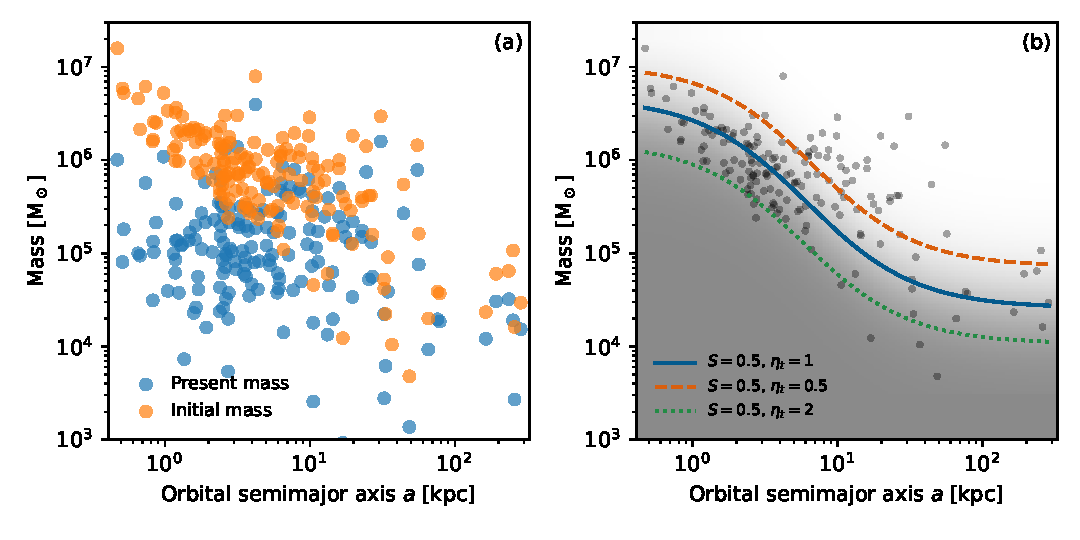
\includegraphics[width=\textwidth]{figures/catalog_mass_semimajor_axis_overview.pdf}
    \caption{Overview of the Baumgardt Milky Way GC catalogue and the adopted smooth survivability model. Left: present-day mass and inferred initial mass as a function of orbital semimajor axis. Right: the fitted smooth survivability surface $S(M_{\rm ini},a)$ for the reference lifetime scale $\eta_t=1$. The solid, dashed, and dotted curves show the fitted $S=0.5$ boundary for $\eta_t=1$, $0.5$, and $2$, respectively. Black points mark the surviving GCs in the catalogue.}
    \label{fig:catalog_overview}\label{fig:survivability}
\end{figure*}

\section{Forward model for the GC catalogue}\label{sec:selection}

The motivation for the model is the strong empirical coupling between GC initial mass and present-day orbit. In the Baumgardt catalogue, the inferred initial masses of surviving Milky Way GCs vary systematically with Galactocentric position, or equivalently with orbital size $a$; this behaviour is already apparent in the discussion of \citet{Baumgardt2019} and fits naturally into the broader post-\textit{Gaia} picture of Galactic assembly reviewed by \citet{DeasonBelokurov2024}. If the Baumgardt initial-mass estimates are trusted as dynamical reconstructions, the surviving clusters provide more than a present-day mass function: they sample the original GC initial mass function down to the lowest initial masses that can still survive to the present day at each orbit size. The task is therefore to model the intrinsic distribution in $(M_{\rm ini},a)$ and then filter it by two effects. The first is dynamical survivability, which we calibrate from the survival times in the Baumgardt calculations. The second is observational detectability, which depends on present-day observables $(l,b,D_\odot,M_{\rm now})$ and is updated iteratively from the model-predicted distribution of GCs in both intrinsic and observable space.

The catalogue contains both intrinsic quantities, which describe the inferred birth mass and orbit of each cluster, and present-day observables, which determine whether a surviving cluster would enter the observed sample. We denote the intrinsic coordinates by
\begin{equation}
x=(\log M_{\rm ini}, \log a),
\end{equation}
and the present-day observable coordinates used in the completeness model by
\begin{equation}
y=(\log M_{\rm now}, \log D_\odot, |b|, |l|).
\end{equation}

A fully marked point-process model would describe the detected catalogue with an intensity
\begin{equation}
\lambda_{\rm det}(x,y)
=
N_0\,\phi(\log M_{\rm ini})\,A(\log a)\,
S(x)\,p(y|x)\,C(y),
\end{equation}
where $\phi$ is the initial mass function, $A$ is the radial birth profile, $S$ is the probability of surviving to the present day, $p(y|x)$ describes the distribution of present-day observables at fixed intrinsic coordinates, and $C$ is the probability that a cluster with observables $y$ is included in the catalogue. In this full model, each observed cluster would contribute its actual present-day observables $y_i$ to the likelihood.

Our implementation uses an intrinsic-space approximation to this marked model. Instead of fitting the full conditional distribution $p(y|x)$ in the likelihood, we average the observable-space completeness over an approximate $p(y|x)$ and define
\begin{equation}
Q(x)=\int p(y|x)\,C(y)\,{\rm d}y.
\end{equation}
The detected intensity in the intrinsic plane is then
\begin{equation}
\lambda_{\rm obs}(x)
=
N_0\,\phi(\log M_{\rm ini})\,A(\log a)\,S(x)\,Q(x).
\end{equation}
Thus $Q$ is the mean detectability of a surviving cluster at a given point in the $(\log M_{\rm ini},\log a)$ plane. This approximation keeps the likelihood two-dimensional while retaining the leading effect of present-day observational incompleteness.

For the observed catalogue $\mathcal{D}=\{x_i\}_{i=1}^{N}$, where $N$ is the number of observed GCs in the working catalogue, the implemented likelihood is the inhomogeneous Poisson likelihood
\begin{equation}
\ln \mathcal{L}
=
\sum_{i=1}^{N} \ln \lambda_{\rm obs}(x_i)
-
\int_{\Omega} \lambda_{\rm obs}(x)\,{\rm d}x,
\end{equation}
Here we omit the Poisson counting term $-\ln N!$ when optimizing models against the same fixed catalogue, since it does not depend on the model parameters. When comparing model classes with different catalogue partitions or label assignments, the corresponding counting terms must be treated consistently. The rest of this section defines the two selection terms, $S$ and $Q$, used in this intrinsic-space likelihood.

\subsection{Survivability}\label{sec:survival}
The observed catalogue is not the IMF itself. It is the subset of clusters that both formed and survived until the present day. We therefore write the first selection term as a survival probability
\begin{equation}
S(\log M_{\rm ini}, a \mid \eta_t).
\end{equation}

The starting point is the analytic dissolution-time prescription used by \citet{Baumgardt2019}. We introduce a dimensionless lifetime-scale parameter $\eta_t$ that multiplies the nominal dissolution rate, or equivalently rescales the age against which the dissolution time is compared. The reference value $\eta_t=1$ corresponds to the unscaled 12 Gyr survival requirement. Values $\eta_t>1$ make clusters longer lived and move the survival boundary to lower initial mass, whereas values $\eta_t<1$ make clusters shorter lived and move the boundary to higher initial mass. For each catalogued GC orbit we compute the threshold mass $M_{\rm cut}(r_{\rm apo}, e)$ that satisfies
\begin{equation}
t_{\rm dis}(M_{\rm cut}, r_{\rm apo}, e)=12\,{\rm Gyr}/\eta_t,
\end{equation}
so changing $\eta_t$ shifts the survivability boundary in the $(M_{\rm ini},a)$ plane.

We first convert the orbit-by-orbit cuts into a raw survivor-based map in $(\log M_{\rm ini}, \log a)$ by kernel-averaging the survival indicators over nearby semimajor axes. This raw map is then regularized into a smooth monotonic family of boundaries $B_{10}(a)$, $B_{50}(a)$, and $B_{90}(a)$ that track the $S=0.1$, $0.5$, and $0.9$ contours. The adopted survivability surface is a logistic transition in $\log M_{\rm ini}$ at fixed semimajor axis,
\begin{equation}
S(m,a)=\left[1+\exp\left(-\frac{m-B_{50}(a)}{\sigma(a)}\right)\right]^{-1},
\end{equation}
with $m\equiv\log M_{\rm ini}$ and
\begin{equation}
\sigma(a)=\frac{B_{90}(a)-B_{10}(a)}{2\ln 9}.
\end{equation}
This construction preserves the calibrated $S=0.1$, $0.5$, and $0.9$ contours and gives a finite, monotonically increasing survival probability throughout the fitted $(M_{\rm ini},a)$ domain.

\subsection{Detectability}\label{sec:detectability}
Survival is not the only filter acting on the GC catalogue. Even among survivors, detectability depends on present-day observables. We therefore introduce a second selection term,
\begin{equation}
C(\log M_{\rm now}, \log D_\odot, |b|, |l|),
\end{equation}
and treat it separately from the dynamical survivability surface.

In the implementation, present-day observable space is binned in $\log M_{\rm now}$, $\log D_\odot$, $|b|$, and $|l|$. The completeness assigned to each bin is written as a logistic function,
\begin{equation}
C = \left[1 + \exp\left(-\beta_0 - s_M z_M + s_D z_D - s_b z_b - s_l z_l\right)\right]^{-1},
\end{equation}
where $z_M$, $z_D$, $z_b$, and $z_l$ are standardized versions of the bin-centred values of $\log M_{\rm now}$, $\log D_\odot$, $|b|$, and $|l|$. The slope parameters are positive by construction, so completeness rises with present-day mass, latitude, and absolute longitude, and falls with heliocentric distance.

To evaluate the effective detectability $Q$, we approximate the conditional distribution $p(y|x)$ rather than fit it as a separate high-dimensional model. We model $\log M_{\rm now}$ using an empirical relation for $\log(M_{\rm now}/M_{\rm ini})$ as a function of $\log M_{\rm ini}$ and $\log a$, including the observed residual scatter when assigning probabilities to present-day mass bins. We then treat $a$ as the characteristic present-day Galactocentric radius of the cluster. At fixed radius $a$, we draw isotropic Galactocentric positions and place the Sun at $R_0=8.2\,\mathrm{kpc}$; this gives the corresponding probability distribution over heliocentric-distance, latitude, and longitude bins. Averaging the binned completeness $C$ over these present-day mass and sky-position probabilities gives the implemented $Q(\log M_{\rm ini},a)$.

Figure~\ref{fig:conditional_observable_approximation} summarizes the present-day mass part of this approximation in the same intrinsic plane used by the likelihood. It compares the observed mass-loss residual, the fitted proxy model, and the remaining per-cluster residuals.

\begin{figure*}
    \centering
    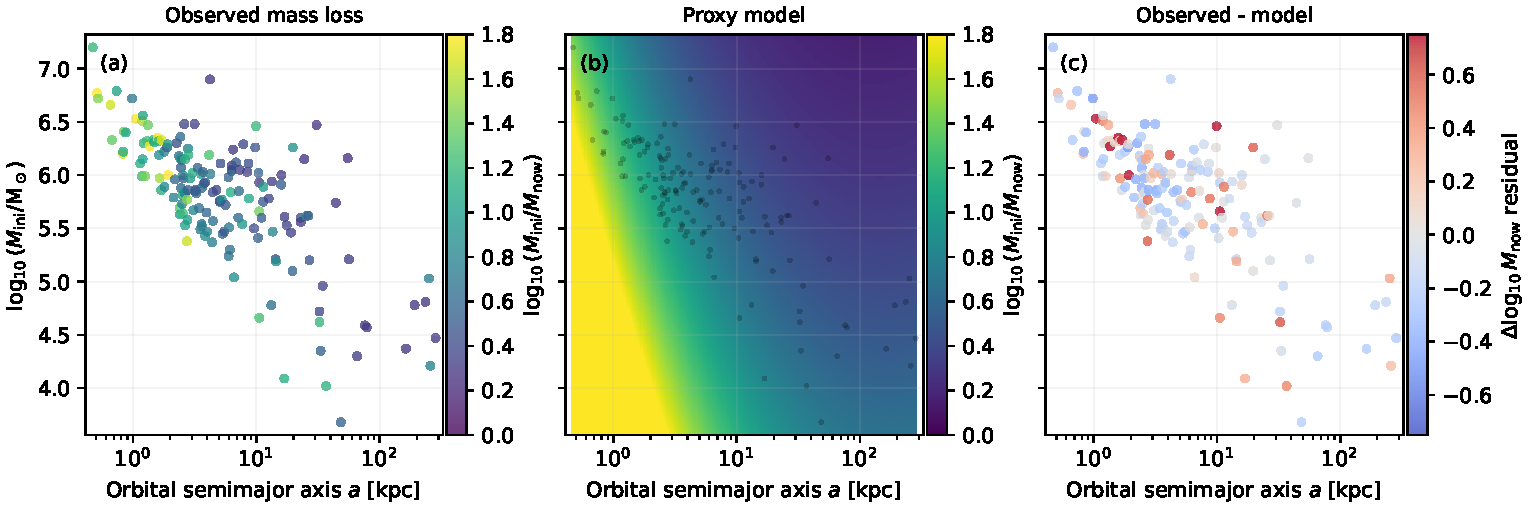
\includegraphics[width=\textwidth]{figures/conditional_observable_approximation.pdf}
    \caption{Present-day mass approximation used when averaging the observable-space completeness into $Q(\log M_{\rm ini},a)$. Left: observed mass-loss residual $\log_{10}(M_{\rm ini}/M_{\rm now})$ in the intrinsic $(M_{\rm ini},a)$ plane. Middle: fitted empirical proxy for the same quantity. Right: per-cluster residuals between the observed and modelled mass-loss residuals. The model is used only to assign probabilities to present-day mass bins at fixed $(M_{\rm ini},a)$; the sky-position part of $p(y|x)$ is computed separately from isotropic Galactocentric positions at fixed $a$.}
    \label{fig:conditional_observable_approximation}
\end{figure*}

Figure~\ref{fig:detectability_em_maps} summarizes the final detectability correction. The one-dimensional panels show how the fitted observable-space completeness $C$ changes with each of its four arguments when the other three are held at representative catalogue values. The lower panel shows the resulting effective detectability $Q(\log M_{\rm ini},a)$ after averaging $C$ over the approximate present-day observable distribution described above.

\begin{figure*}
    \centering
    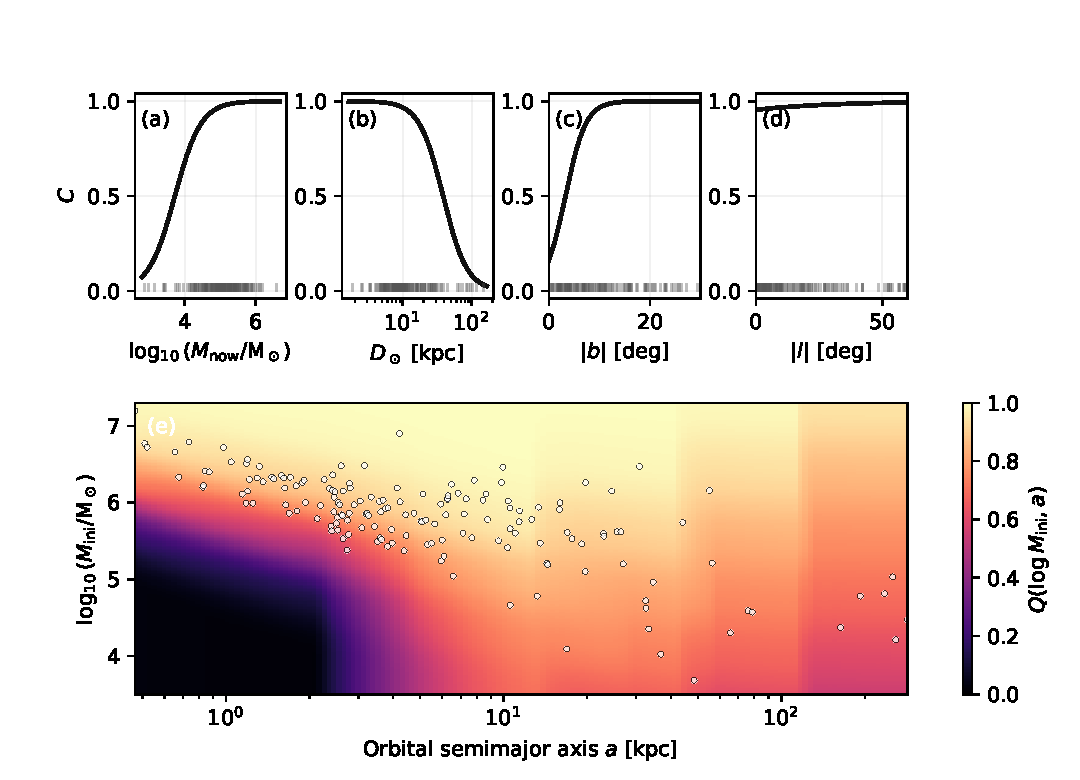
\includegraphics[width=\textwidth]{figures/detectability_em_maps.pdf}
    \caption{Detectability correction used by the adopted intrinsic-space likelihood. Top: response curves of the fitted observable-space completeness law $C(\log M_{\rm now},\log D_\odot,|b|,|l|)$, varying one observable at a time while holding the others fixed at their catalogue medians. Rug marks show the observed catalogue values along each axis. Bottom: effective detectability $Q(\log M_{\rm ini},a)$ obtained by averaging $C$ over the approximate conditional distribution of present-day observables at fixed intrinsic coordinates. White points mark the observed GCs.}
    \label{fig:detectability_em_maps}
\end{figure*}

\section{Single-component implementation}\label{sec:model_single}
For the single-component model used in this paper, the IMF factor $\phi$ in the intrinsic intensity is a Schechter function with slope $\alpha$ and cutoff mass $M_c$, normalized over the fitted range in $\log M_{\rm ini}$. The radial birth factor $A$ is a normalized function of $\log a$; our preferred family is the smooth cubic polynomial $\texttt{logpoly3}$, but we also compare against a five-bin step model, a single power law in $a$, and a cored power law $dN/da\propto(a+a_c)^{-\gamma}$. The total normalization $N_0$ is the inferred number of initial clusters over the fitted domain. With these definitions, all likelihood evaluations use the intrinsic-space intensity defined in Section~\ref{sec:selection}.

\subsection{Iterative detectability correction}\label{sec:detectability_algorithm}
The detectability term is solved with an iterative detectability correction. At fixed outer parameters $(\eta_t,\alpha,\log_{10}M_c)$ we:
\begin{enumerate}
    \item build the smooth survivability surface $S(M_{\rm ini},a\mid\eta_t)$;
    \item fit the baseline single-component model assuming $Q=1$;
    \item project the resulting complete surviving population into $(\log M_{\rm now}, \log D_\odot, |b|, |l|)$;
    \item fit the logistic completeness law in observable space;
    \item average that completeness back into intrinsic space to obtain $Q(M_{\rm ini},a)$;
    \item refit the intrinsic model and repeat until convergence.
\end{enumerate}
The profiling uses 12 such iterations at each outer trial point. In practice the detectability update converges quickly in the high-likelihood region of parameter space. Figure~\ref{fig:detectability_em_convergence} shows an unfiltered grid of representative inner solves for trial outer parameters near the preferred region, extended to 30 iterations as a diagnostic. Two behaviours are apparent. Some trials stabilize rapidly: the inferred normalization, mean detectability, predicted observed count, and profiled intrinsic likelihood change little after this iteration count. Other trials drift toward very low effective detectability and very large normalization; these are low-likelihood self-consistent corrections associated with poor outer parameters. They are not removed by hand, but are retained as likelihood evaluations and are naturally disfavoured by the outer profile likelihood. The likelihood sequence is not constrained to increase at every step: at each step the inner fit optimizes the likelihood for the current fixed $Q$, whereas the next step changes $Q$ itself.

\begin{figure}
    \centering
    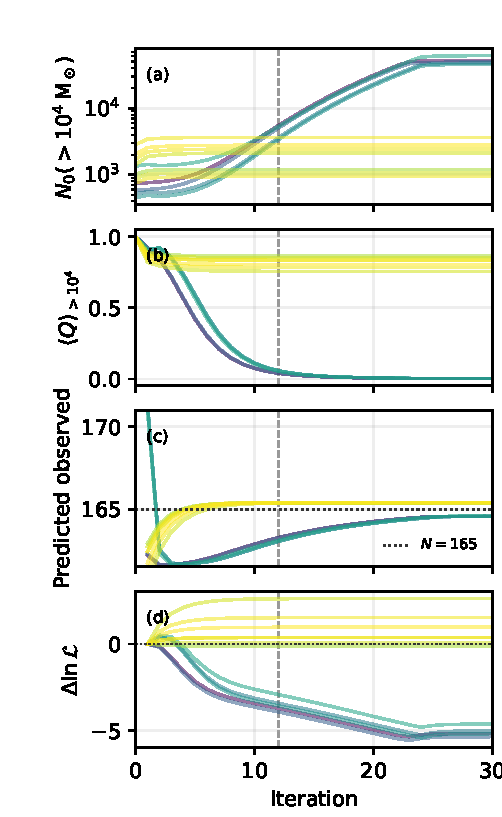
\includegraphics[width=\columnwidth]{figures/detectability_em_convergence.pdf}
    \caption{Unfiltered grid of representative inner solves for the iterative detectability correction at fixed trial outer parameters near the preferred region, shown for 30 iterations. Each transparent line is one solve, with the same colour used across all panels; the colour ordering follows the final profiled log-likelihood of the solve. The vertical dashed line marks the 12 iterations used in profiling. The panels show the inferred initial count above $M_{\rm ini}=10^4\,{\rm M}_\odot$, the mean effective detectability above the same mass, the predicted observed catalogue size, and the change in profiled intrinsic log-likelihood relative to the first iteration of each solve.}
    \label{fig:detectability_em_convergence}
\end{figure}

\subsection{Exact profiling and MCMC}\label{sec:optimization}
The expensive part of the problem is not the Schechter IMF itself, but the nested profiling over the radial law, detectability correction, and normalization. We therefore separate the inference into outer physical parameters and inner nuisance parameters.

The outer parameter vector is
\begin{equation}
\theta_{\rm out}=(\eta_t,\alpha,\log_{10}M_c).
\end{equation}
For every proposed $\theta_{\rm out}$ we rebuild the survivability surface, run the iterative detectability correction, and profile over the $\texttt{logpoly3}$ radial parameters and the total normalization. The inner solve is deterministic: every likelihood evaluation uses the same restart library and optimization settings, so the outer likelihood does not depend on chain history.

We first map the likelihood surface with a broad exact coarse scan, then refine the high-likelihood region. After locating the main ridge we run exact parallel profiled MCMC in the three outer parameters only, profiling over the nuisance parameters at every step. The production run used six chains of 900 steps each, with a burn-in of 300 steps and thinning by a factor of 2. Figure~\ref{fig:single_component_posterior} shows the corresponding exact profiled posterior.

\begin{figure*}
    \centering
    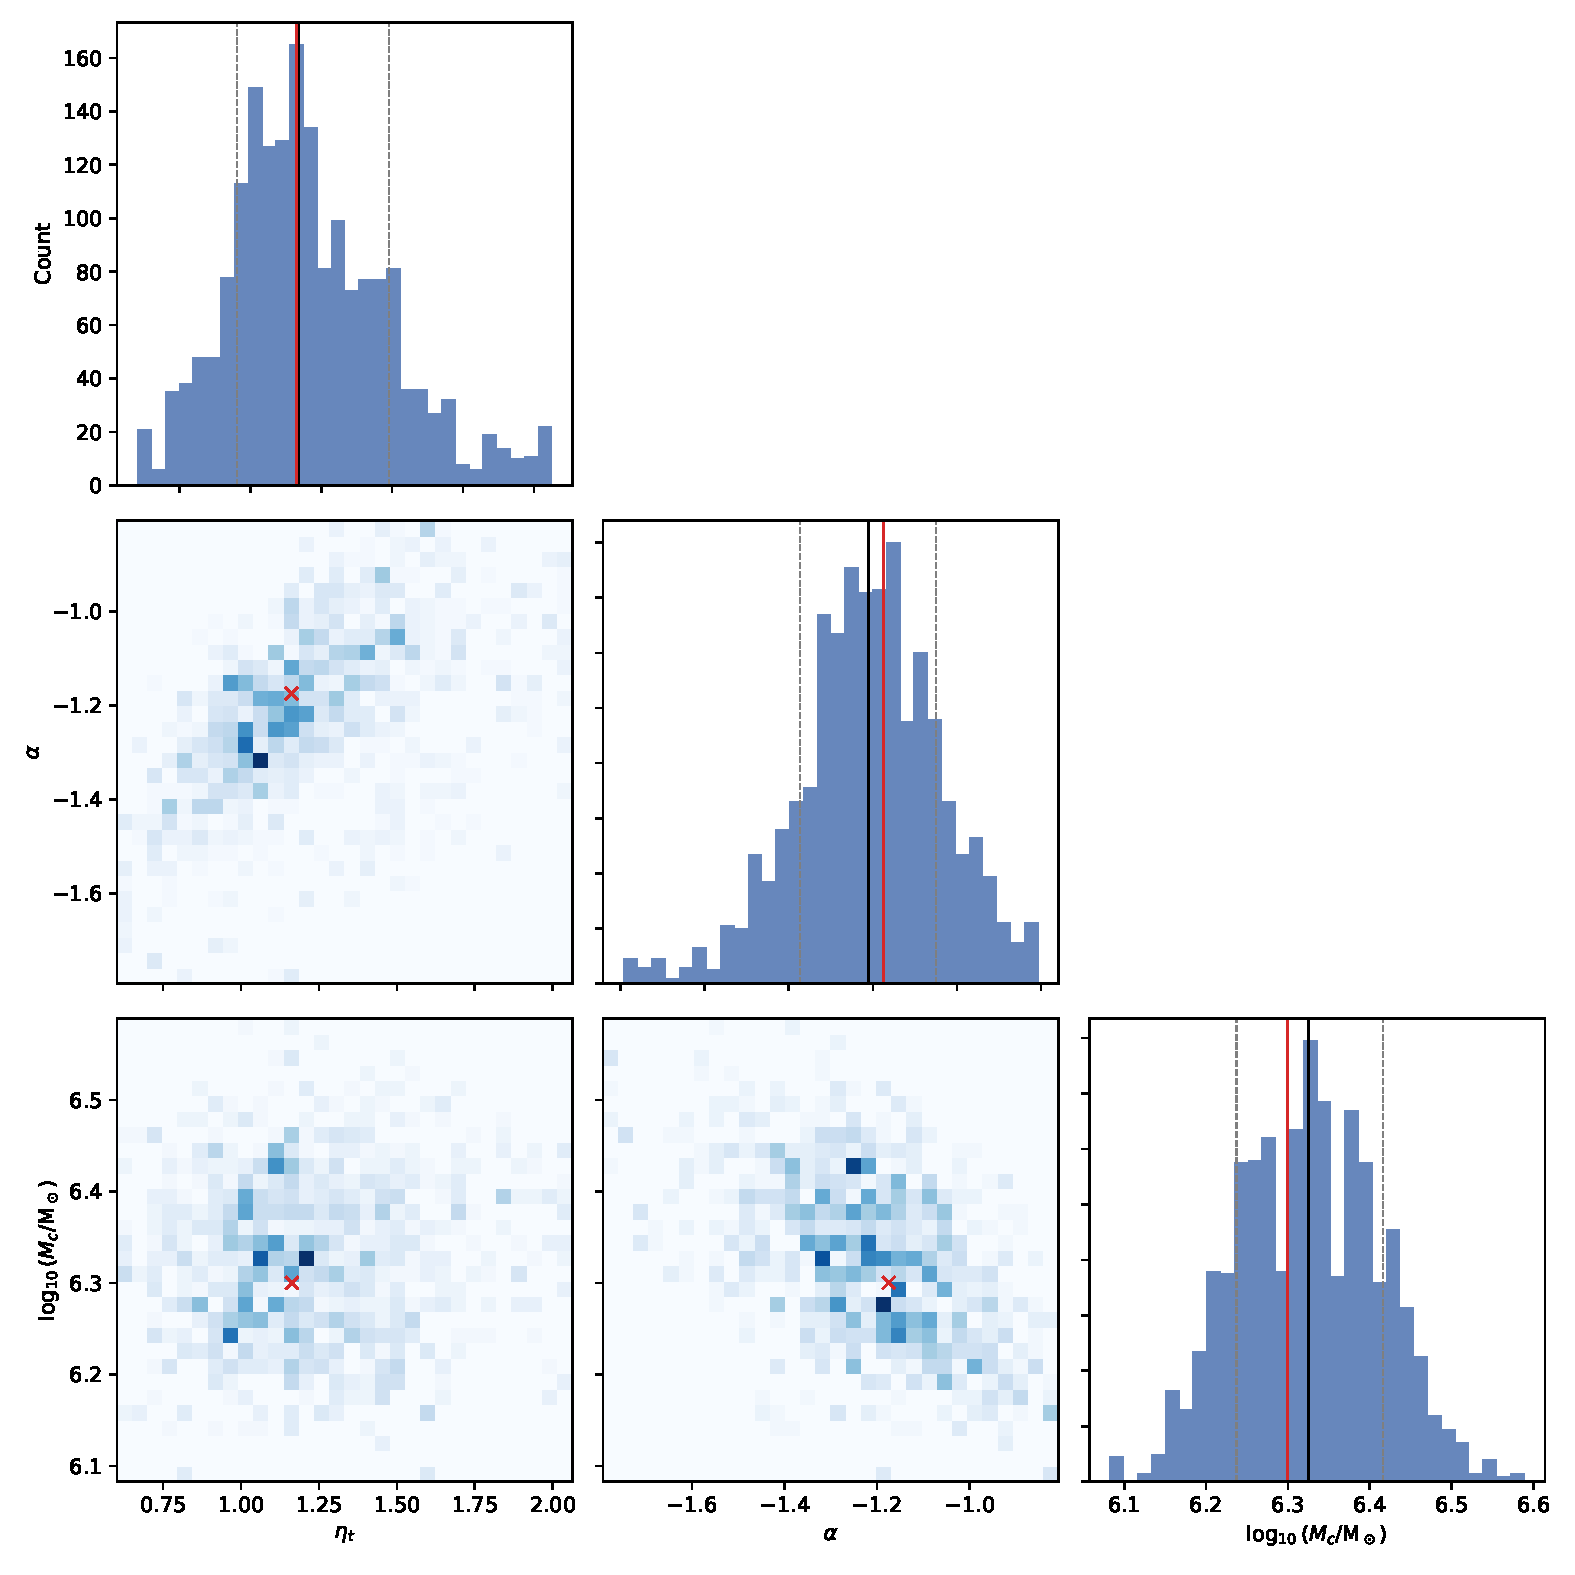
\includegraphics[width=0.72\textwidth]{figures/single_component_posterior_corner.pdf}
    \caption{Exact profiled posterior for the three outer physical parameters $(\eta_t,\alpha,\log_{10}M_c)$ in the adopted single-component model. The inner radial and detectability nuisance parameters are re-optimized at every step, so the plotted posterior is the true profiled posterior in the outer physical parameter space.}
    \label{fig:single_component_posterior}
\end{figure*}

\subsection{Single-component results}\label{sec:single_component_results}
The preferred single-component model uses the smooth $\texttt{logpoly3}$ radial family. Its best-fit parameters are
\begin{equation}
\eta_t=\ExactBestEta,
\qquad
\alpha=\ExactBestAlpha,
\qquad
\log_{10}(M_c/{\rm M}_\odot)=\ExactBestMc,
\end{equation}
with $\log\mathcal{L}=\ExactBestLogL$. The corresponding exact profiled MCMC gives
\begin{equation}
\eta_t = \PosteriorEtaMed_{-\PosteriorEtaMinus}^{+\PosteriorEtaPlus},
\end{equation}
\begin{equation}
\alpha = \PosteriorAlphaMed_{-\PosteriorAlphaMinus}^{+\PosteriorAlphaPlus},
\end{equation}
\begin{equation}
\log_{10}(M_c/{\rm M}_\odot)=\PosteriorMcMed_{-\PosteriorMcMinus}^{+\PosteriorMcPlus}.
\end{equation}
Above $M_{\rm ini}=10^4\,{\rm M}_\odot$, the inferred initial population is
\begin{equation}
N_0 = \PosteriorNzeroMed_{-\PosteriorNzeroMinus}^{+\PosteriorNzeroPlus},
\end{equation}
corresponding to a total initial stellar mass of
\begin{equation}
M_{\star,0}=\PosteriorMassZeroEightMed_{-\PosteriorMassZeroEightMinus}^{+\PosteriorMassZeroEightPlus}\times10^8\,{\rm M}_\odot.
\end{equation}
The mean detectability of the surviving population is
\begin{equation}
\langle Q\rangle_{S,M>10^4} = \PosteriorMeanDetectabilityMed_{-\PosteriorMeanDetectabilityMinus}^{+\PosteriorMeanDetectabilityPlus}.
\end{equation}
This is an average over the model-predicted surviving population above $10^4\,{\rm M}_\odot$, not an area average of the $Q(\log M_{\rm ini},a)$ map and not an average over only the observed catalogue. Relative to the same-Schechter perfect-detectability baseline at the best-fit outer parameters, the detectability correction raises the inferred normalization from $N_0=\ExactBaselineNzero$ to $N_0=\ExactBestNzero$, a factor of \ExactCountRatio.

Figure~\ref{fig:survivability_detectability_mass_profiles} shows the same selection terms collapsed as functions of initial mass. The left panel shows
\begin{equation}
\langle S\rangle_{\rho(a)}(\log M_{\rm ini}) =
\int S(\log M_{\rm ini},a)\,\rho(a)\,d\log a ,
\end{equation}
where $\rho(a)$ is the fitted intrinsic radial birth profile. The right panel shows
\begin{equation}
\begin{aligned}
\langle Q\rangle_{\rho S}(\log M_{\rm ini})
&= \frac{\int Q(\log M_{\rm ini},a)\,w_S\,d\log a}
        {\int w_S\,d\log a},\\
w_S(\log M_{\rm ini},a)
&= S(\log M_{\rm ini},a)\,\rho(a).
\end{aligned}
\end{equation}
Thus the detectability curve is not averaged over all radii at fixed mass. It is averaged over the clusters that survive at that mass.

This distinction is important. The two-dimensional $Q$ map in Figure~\ref{fig:detectability_em_maps} contains low-detectability regions in the inner Galaxy, especially at low present-day mass. However, these are also the regions where the survivability surface removes a large fraction of the initial population. In the adopted model, low-mass clusters born at small $a$ rarely survive to the present day; the surviving inner clusters are biased toward higher initial mass, where the present-day mass proxy gives higher detectability. At larger $a$, lower-mass survivors are more common, but their sky-averaged detectability is also higher. The scalar $\langle Q\rangle_{S,M>10^4}$ is therefore high because it is a survivor-weighted average. It measures the completeness of the surviving population predicted by the model, not the completeness of all initial clusters and not the visual area covered by the $Q(\log M_{\rm ini},a)$ map.

\begin{figure}
    \centering
    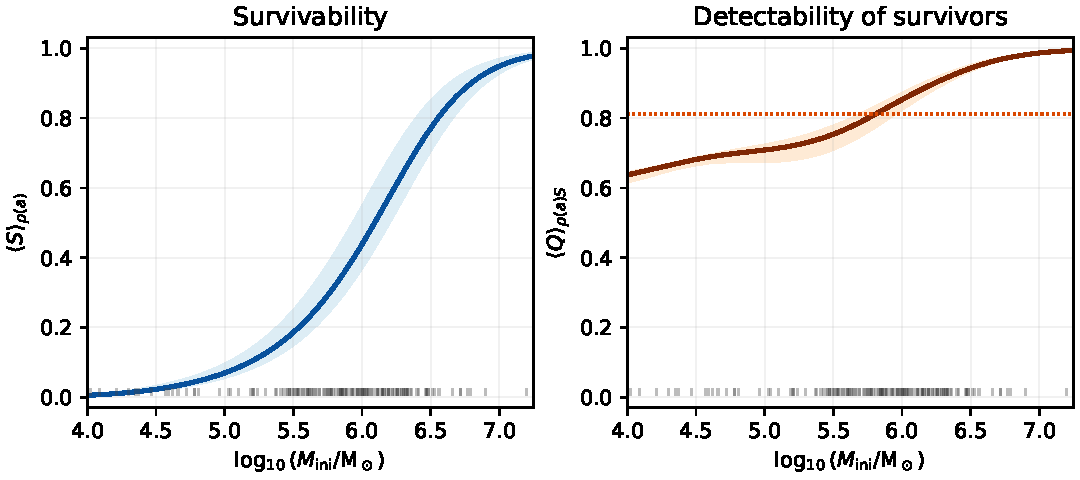
\includegraphics[width=\columnwidth]{figures/survivability_detectability_mass_profiles.pdf}
    \caption{Mass dependence of the two selection factors in the adopted exact single-component fit. Left: radial-profile-weighted survivability, $\langle S\rangle_{\rho(a)}$. Right: detectability averaged over the surviving population at fixed initial mass, $\langle Q\rangle_{\rho(a)S}$; the dotted horizontal line marks the posterior median of the scalar survivor-weighted mean $\langle Q\rangle_{S,M>10^4}$. Solid curves show the best profiled model. Shaded bands show the central 68 per cent range from the stored posterior $S$ and $Q$ surface samples, with the best-fit radial weighting held fixed. The high value of the scalar mean reflects the ordering of the two selection effects: many low-mass inner clusters occupy low-$Q$ regions but also have low survivability, so they carry little weight in the survivor-weighted average.}
    \label{fig:survivability_detectability_mass_profiles}
\end{figure}

Figure~\ref{fig:single_component_intensity_plane} shows the adopted relative detected probability density in the $(M_{\rm ini},a)$ plane, and Figure~\ref{fig:best_single_component} shows its one-dimensional projections together with the residual map. The preferred model follows the observed catalogue well with a moderate detectability correction and a total inferred population of order $\PosteriorNzeroMed$ clusters above $10^4\,{\rm M}_\odot$.

\begin{figure}
    \centering
    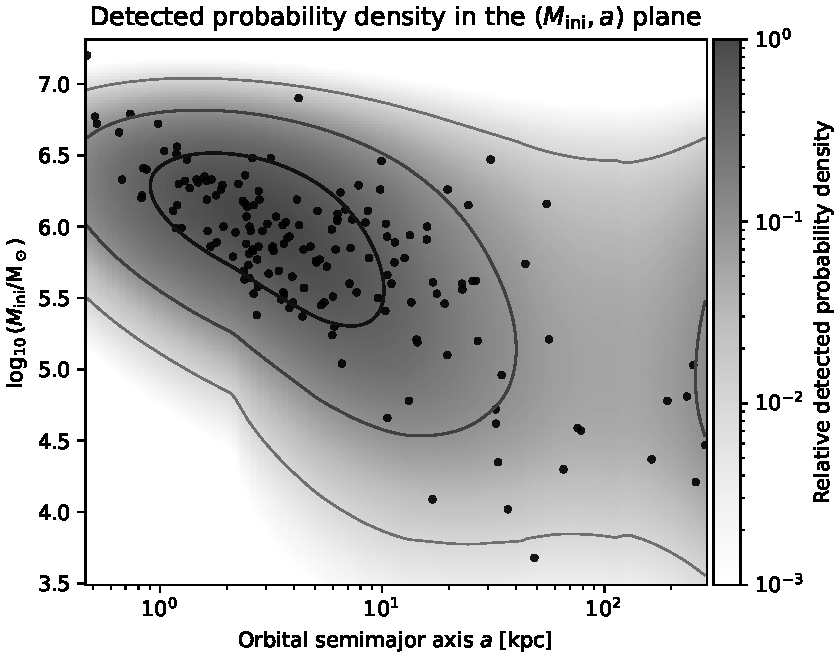
\includegraphics[width=\columnwidth]{figures/single_component_intensity_plane.pdf}
    \caption{Relative detected probability density in the $(M_{\rm ini},a)$ plane for the adopted exact single-component model, with the surviving clusters overplotted in black. Darker greyscale values indicate higher probability density, and the contours mark relative density levels of 0.01, 0.1, and 0.5. This is the standalone version of the intrinsic-plane panel that used to be embedded in the multi-panel summary figure.}
    \label{fig:single_component_intensity_plane}
\end{figure}

\begin{figure*}
    \centering
    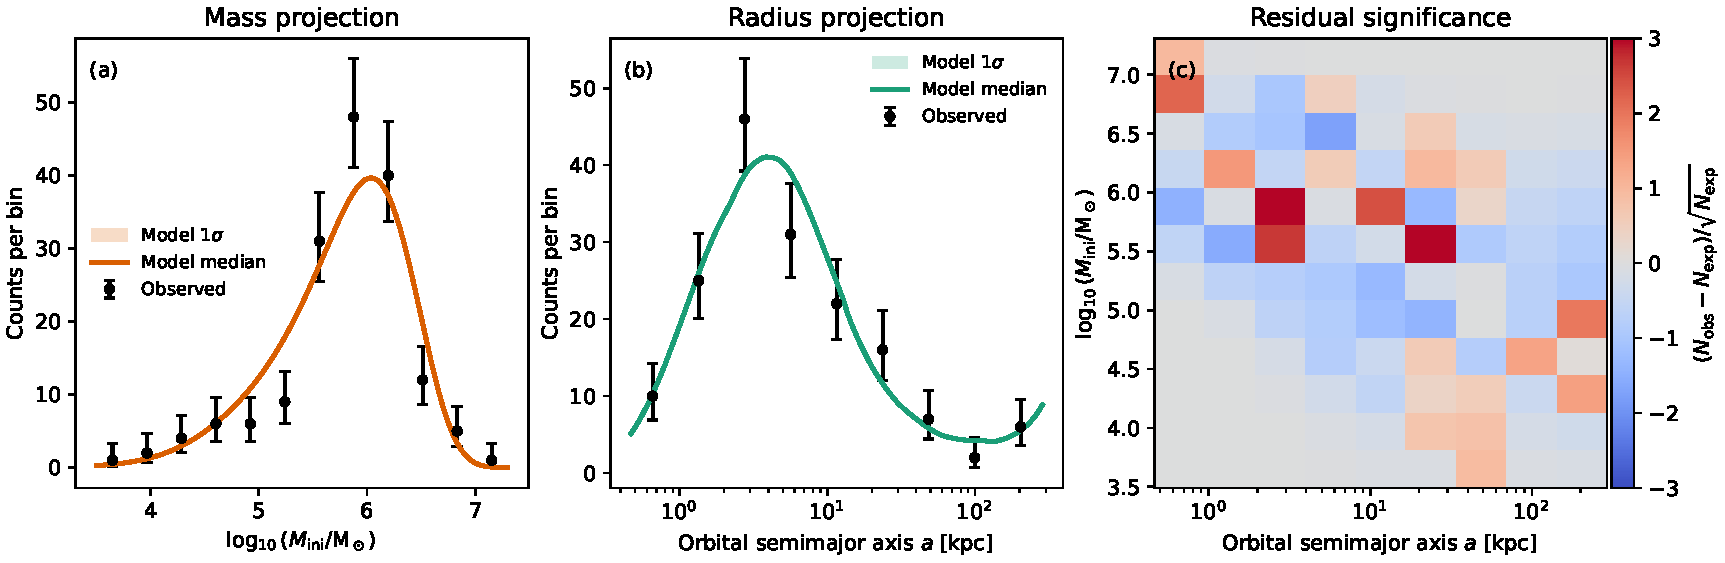
\includegraphics[width=\textwidth]{figures/best_single_component_summary.pdf}
    \caption{Three-panel summary of the adopted exact single-component model. Left: the projected initial-mass distribution. Middle: the projected semimajor-axis distribution. Right: residual significance in coarse bins of the $(M_{\rm ini},a)$ plane. The line predictions use the best profiled monotonic-$Q$ solution.}
    \label{fig:best_single_component}
\end{figure*}

Figure~\ref{fig:single_component_profiles} shows the inferred Schechter IMF with a truthful posterior band built directly from the exact profiled posterior samples. Because the band is constructed from the posterior samples themselves rather than from a local covariance approximation, it captures both the uncertainty in slope and cutoff mass and the uncertainty in the normalization above $10^4\,{\rm M}_\odot$.

\begin{figure}
    \centering
    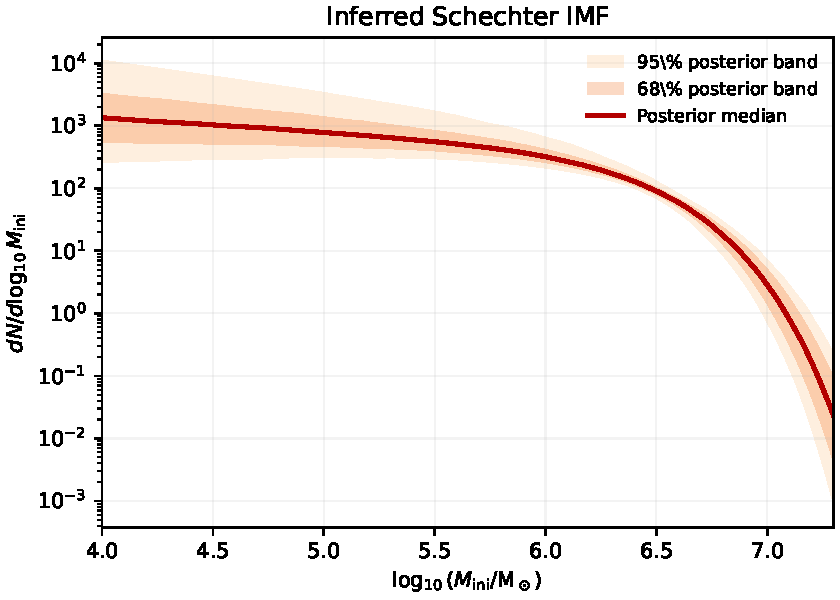
\includegraphics[width=\columnwidth]{figures/single_component_profiles.pdf}
    \caption{Inferred Schechter IMF for the adopted exact single-component model, shown only for $M_{\rm ini}\ge10^4\,{\rm M}_\odot$. The dark curve is the posterior median and the shaded regions show the 68 and 95 per cent posterior bands obtained directly from the exact profiled MCMC samples.}
    \label{fig:single_component_profiles}
\end{figure}

The radial model comparison is shown in Figure~\ref{fig:single_component_radial_profile}. On the same exact footing, the smooth $\texttt{logpoly3}$ family outperforms all three alternatives. Relative to the preferred model, the five-bin step model is worse by $\Delta\mathrm{AIC}=\StepFiveDeltaAIC$ and $\Delta\mathrm{BIC}=\StepFiveDeltaBIC$, while the single power law in $a$ is worse by $\Delta\mathrm{AIC}=\PowerLawADeltaAIC$ and $\Delta\mathrm{BIC}=\PowerLawADeltaBIC$. The cored power law performs better than either of these simpler alternatives, with $\Delta\mathrm{AIC}=\CoredPowerLawADeltaAIC$ and $\Delta\mathrm{BIC}=\CoredPowerLawADeltaBIC$, but it remains disfavoured relative to $\texttt{logpoly3}$. Its posterior radial parameters are $\gamma=\CoredPowerLawAGammaMed_{-\CoredPowerLawAGammaMinus}^{+\CoredPowerLawAGammaPlus}$ and $a_c=\CoredPowerLawACoreKpcMed_{-\CoredPowerLawACoreKpcMinus}^{+\CoredPowerLawACoreKpcPlus}\,{\rm kpc}$. The preference for $\texttt{logpoly3}$ is therefore not just visual; it survives the explicit complexity penalty as well.

\begin{figure*}
    \centering
    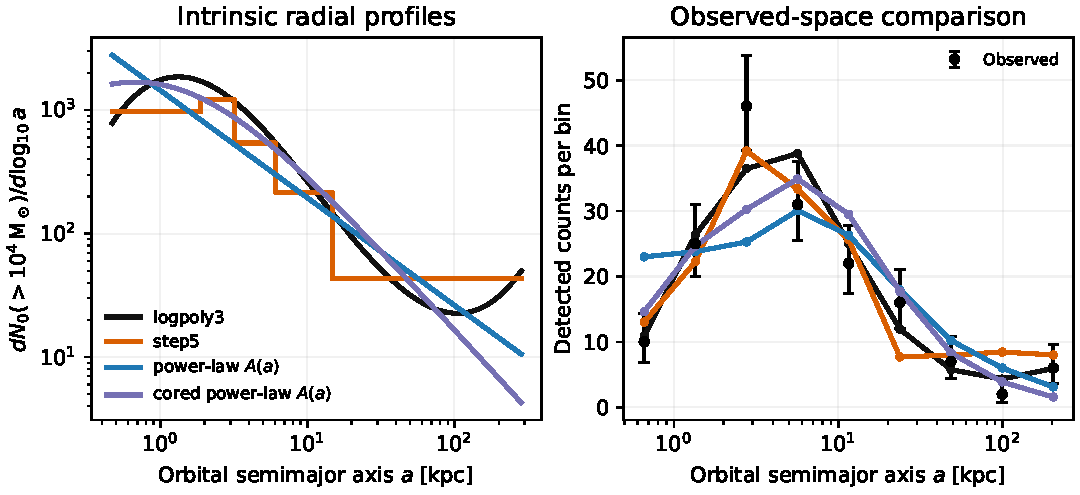
\includegraphics[width=\textwidth]{figures/single_component_radial_profile.pdf}
    \caption{Radial-model comparison under the same logistic-tail survivability model and the same exact profiled Schechter framework. Left: inferred intrinsic radial profiles, shown as the initial number of clusters above $10^4\,{\rm M}_\odot$ per dex in semimajor axis. Right: observed semimajor-axis counts compared to the corresponding detected-count predictions. The preferred $\texttt{logpoly3}$ family fits the observed radial counts better than the five-bin step model, the single power law in $a$, and the cored power law in $a$.}
    \label{fig:single_component_radial_profile}
\end{figure*}

\clearpage

\section{Two-component model with Belokurov--Kravtsov labels}\label{sec:two_component}
We next fit a labelled two-component extension using the in-situ/accreted assignments of \citet{BelokurovKravtsov2024}. The labels are treated as fixed data, not inferred mixture memberships. Thus the model asks whether the same IMF, filtered through two different radial birth profiles, gives a better description of the labelled catalogue.

Let $g\in\{\mathrm{in},\mathrm{acc}\}$ denote the Belokurov--Kravtsov label. The two component intensities are
\begin{equation}
\lambda_g(x)
=
N_{0,g}\,\phi(\log M_{\rm ini}\mid \alpha,M_c)\,
A_g(\log a)\,S(x\mid\eta_t)\,Q(x),
\end{equation}
where the Schechter IMF parameters $(\alpha,\log_{10}M_c)$ and survivability parameter $\eta_t$ are shared, while each component has its own normalized smooth $\texttt{logpoly3}$ radial profile $A_g$ and normalization $N_{0,g}$. The detectability term $Q$ is the same intrinsic-space approximation defined in Section~\ref{sec:detectability}; the completeness law is fitted to the pooled observed catalogue and then applied to both labelled components. The labelled point-process likelihood is
\begin{equation}
\ln \mathcal{L}_{2}
=
\sum_g
\left[
\sum_{i\in g}\ln\lambda_g(x_i)
-
\int_\Omega \lambda_g(x)\,{\rm d}x
-
\ln N_g!
\right],
\end{equation}
with $N_{\rm in}=\TwoCompNInSitu$, $N_{\rm acc}=\TwoCompNAccreted$, and $N=\TwoCompNTotal$.

The factorial term matters for comparing the labelled two-component model to the unlabelled single-component model. The single-component likelihood contains $-\ln N!$, whereas the fixed labelled likelihood contains $-\ln N_{\rm in}!-\ln N_{\rm acc}!$. If the parameter-independent constants have been dropped during optimization, the labelled two-component likelihood must therefore be shifted onto the single-catalogue scale by
\begin{equation}
C_{\rm part}
=
\ln\frac{N!}{N_{\rm in}!\,N_{\rm acc}!}
=\TwoCompPartitionConstant .
\end{equation}
Equivalently,
\begin{align}
\ln\mathcal{L}_{2,\mathrm{cond}}
&=
\ln\mathcal{L}_{2,\mathrm{raw}}+C_{\rm part},\\
\mathrm{BIC}_{2,\mathrm{cond}}
&=
\mathrm{BIC}_{2,\mathrm{raw}}-2C_{\rm part}.
\end{align}
This correction does not affect the posterior within the two-component model, but it is required for any one- versus two-component $\Delta\mathrm{BIC}$. With the convention $\Delta\mathrm{BIC}=\mathrm{BIC}_{2}-\mathrm{BIC}_{1}$, the raw comparison gives $\Delta\mathrm{BIC}_{\rm raw}=\TwoCompRawDeltaBIC$, while the fixed-label correction gives $\Delta\mathrm{BIC}_{\rm cond}=\TwoCompConditionalDeltaBIC$. The corrected number should be interpreted as support for the imposed Belokurov--Kravtsov radial split, not as a blind discovery of two populations.

Table~\ref{tab:two_component_check} summarizes the exact profiled MCMC result. The shared outer-parameter posterior is almost unchanged relative to the single-component fit. The two-component run gives $\eta_t=\TwoCompEtaMed_{-\TwoCompEtaMinus}^{+\TwoCompEtaPlus}$, $\alpha=\TwoCompAlphaMed_{-\TwoCompAlphaMinus}^{+\TwoCompAlphaPlus}$, and $\log_{10}(M_c/{\rm M}_\odot)=\TwoCompMcMed_{-\TwoCompMcMinus}^{+\TwoCompMcPlus}$, consistent with the single-component posterior. The total inferred population above $10^4\,{\rm M}_\odot$ is also similar, $N_0=\TwoCompNzeroMed_{-\TwoCompNzeroMinus}^{+\TwoCompNzeroPlus}$.

The useful new information is the decomposition of this lower bound. The accreted-labelled clusters contribute $N_{0,\rm acc}=\TwoCompAccretedNzeroMed_{-\TwoCompAccretedNzeroMinus}^{+\TwoCompAccretedNzeroPlus}$ above $10^4\,{\rm M}_\odot$, corresponding to an accreted fraction $f_{\rm acc}=\TwoCompAccretedFractionMed_{-\TwoCompAccretedFractionMinus}^{+\TwoCompAccretedFractionPlus}$. Most of the broad high-normalization tail therefore remains attached to the in-situ-labelled component, not to the accreted-labelled one. Since the labels are imposed rather than inferred, this result is best read as a labelled decomposition of the single-component solution: allowing the Belokurov--Kravtsov components to have separate radial profiles does not move the inferred Schechter IMF appreciably.

\begin{table*}
    \centering
    \caption{Exact profiled MCMC comparison between the adopted single-component model and the labelled Belokurov--Kravtsov two-component diagnostic. Quoted intervals are the central 68 per cent posterior ranges. The two-component model has a shared Schechter IMF and separate $\texttt{logpoly3}$ radial profiles for the fixed in-situ and accreted labels.}
    \label{tab:two_component_check}
    \begin{tabular}{lcccc}
        \hline
        % Generated by scripts/build_two_component_paper_tables.py.
% This file is the body of Table~\ref{tab:two_component_check}.
Quantity & Single component & Two-component total & In situ & Accreted \\
\hline
$\eta_t$ & $\PosteriorEtaMed_{-\PosteriorEtaMinus}^{+\PosteriorEtaPlus}$ & $\TwoCompEtaMed_{-\TwoCompEtaMinus}^{+\TwoCompEtaPlus}$ & -- & -- \\
$\alpha$ & $\PosteriorAlphaMed_{-\PosteriorAlphaMinus}^{+\PosteriorAlphaPlus}$ & $\TwoCompAlphaMed_{-\TwoCompAlphaMinus}^{+\TwoCompAlphaPlus}$ & -- & -- \\
$\log_{10}(M_c/{\rm M}_\odot)$ & $\PosteriorMcMed_{-\PosteriorMcMinus}^{+\PosteriorMcPlus}$ & $\TwoCompMcMed_{-\TwoCompMcMinus}^{+\TwoCompMcPlus}$ & -- & -- \\
$N_0(>10^4\,{\rm M}_\odot)$ & $\PosteriorNzeroMed_{-\PosteriorNzeroMinus}^{+\PosteriorNzeroPlus}$ & $\TwoCompNzeroMed_{-\TwoCompNzeroMinus}^{+\TwoCompNzeroPlus}$ & $\TwoCompInSituNzeroMed_{-\TwoCompInSituNzeroMinus}^{+\TwoCompInSituNzeroPlus}$ & $\TwoCompAccretedNzeroMed_{-\TwoCompAccretedNzeroMinus}^{+\TwoCompAccretedNzeroPlus}$ \\
$M_{\star,0}(>10^4\,{\rm M}_\odot)\,[10^8\,{\rm M}_\odot]$ & $\PosteriorMassZeroEightMed_{-\PosteriorMassZeroEightMinus}^{+\PosteriorMassZeroEightPlus}$ & $\TwoCompMassZeroEightMed_{-\TwoCompMassZeroEightMinus}^{+\TwoCompMassZeroEightPlus}$ & $\TwoCompInSituMassZeroEightMed_{-\TwoCompInSituMassZeroEightMinus}^{+\TwoCompInSituMassZeroEightPlus}$ & $\TwoCompAccretedMassZeroEightMed_{-\TwoCompAccretedMassZeroEightMinus}^{+\TwoCompAccretedMassZeroEightPlus}$ \\
$\langle Q\rangle_{>10^4}$ & $\PosteriorMeanDetectabilityMed_{-\PosteriorMeanDetectabilityMinus}^{+\PosteriorMeanDetectabilityPlus}$ & $\TwoCompMeanDetectabilityMed_{-\TwoCompMeanDetectabilityMinus}^{+\TwoCompMeanDetectabilityPlus}$ & -- & -- \\
$f_{\rm acc}$ & -- & $\TwoCompAccretedFractionMed_{-\TwoCompAccretedFractionMinus}^{+\TwoCompAccretedFractionPlus}$ & -- & -- \\
\hline

    \end{tabular}
\end{table*}

\clearpage

\section{Initial masses under the Gieles--Gnedin disruption law}\label{sec:gg23_masses}
The preceding inference uses the Baumgardt initial masses and the Baumgardt-based survivability surface as the baseline coordinate system. It is useful to ask how much of the result depends on that particular disruption calibration. As a first controlled comparison, we recompute the cluster initial masses and survivability boundaries using the analytic mass-loss law of \citet{GielesGnedin2023}, hereafter GG23.

GG23 write the evaporation-driven mass-loss rate as
\begin{equation}
\dot{M}
=
\dot{M}_{\rm ref}
\left(\frac{M}{M_{\rm ini}}\right)^{1-y}
\left(\frac{M_{\rm ini}}{2\times10^5\,{\rm M}_\odot}\right)^{1-x}
\frac{\Omega_{\rm tid}}{0.32\,{\rm Myr}^{-1}},
\end{equation}
with $x=2/3$. Integrating this law gives
\begin{equation}
M(t)=M_{\rm ini}
\left[
1-\frac{t}{t_{\rm dis}(M_{\rm ini},\Omega_{\rm tid})}
\right]^{1/y},
\end{equation}
where
\begin{equation}
\begin{aligned}
t_{\rm dis}
&=
10\,{\rm Gyr}\,
\frac{2/3}{y}\,
\frac{30\,{\rm M}_\odot\,{\rm Myr}^{-1}}{|\dot{M}_{\rm ref}|}\,
\frac{0.32\,{\rm Myr}^{-1}}{\Omega_{\rm tid}}\\
&\quad\times
\left(\frac{M_{\rm ini}}{2\times10^5\,{\rm M}_\odot}\right)^x .
\end{aligned}
\end{equation}
We have checked this implementation against the public \texttt{evgcmf.py} code associated with GG23: for fixed $M_{\rm ini}$, gradient radius, and effective tidal radius, the local calculation agrees with the GG23 equations at machine precision for the survival threshold, disruption time, and evolved present-day mass.

To apply this law to the Milky Way catalogue we need a two-dimensional projection into the same $(M_{\rm ini},a)$ plane used throughout the paper. For each cluster we approximate the effective tidal radius by
\begin{equation}
R_{\rm eff}=a(1-e^2),
\end{equation}
equivalent to $R_p(1+e)$ for an orbit with semimajor axis $a$ and eccentricity $e$. The tidal frequency is then scaled as $\Omega_{\rm tid}=0.32\,{\rm Myr}^{-1}(R_{\rm eff}/{\rm kpc})^{-1}$ for the reference circular speed $V_c=220\,{\rm km\,s^{-1}}$. For the GG23 metallicity-gradient variants we use the GG23 radial prescription,
\begin{align}
\dot{M}_{\rm ref}(R)&=-30\,{\rm M}_\odot\,{\rm Myr}^{-1}
\left[1+\frac{1}{2}\log_{10}\left(\frac{R}{{\rm kpc}}\right)\right],\\
y(R)&=\frac{2}{3}+\frac{2}{3}\log_{10}\left(\frac{R}{{\rm kpc}}\right),
\end{align}
for $R<10\,{\rm kpc}$, and $\dot{M}_{\rm ref}=-45\,{\rm M}_\odot\,{\rm Myr}^{-1}$, $y=4/3$ at larger radii. In the projected catalogue calculation we set this gradient radius to $R\simeq a$. For the past-tidal-evolution variants we multiply $|\dot{M}_{\rm ref}|$ by $(R_{\rm eff}/4\,{\rm kpc})^{1/2}$ when $R_{\rm eff}>4\,{\rm kpc}$, following GG23.

For each observed cluster and each GG23 variant, we infer an alternative initial mass by solving
\begin{equation}
M_{\rm now}
=
M_{\rm ini}^{\rm GG23}
\left[
1-\frac{12\,{\rm Gyr}}
{t_{\rm dis}(M_{\rm ini}^{\rm GG23},R_{\rm eff},R)}
\right]^{1/y(R)}
\end{equation}
for $M_{\rm ini}^{\rm GG23}$. This scalar inversion is monotonic above the disruption threshold, so a bracketed numerical solve is stable. Forward-evolving the recovered masses returns the observed present-day masses with fractional residuals below $1.5\times10^{-9}$ for all five GG23 variants.

Figure~\ref{fig:gg23_initial_mass_comparison} compares these GG23 initial masses to the Baumgardt values. The no-BH prescription gives systematically smaller initial masses, with a median offset of about $-0.34$ dex relative to Baumgardt. The BH-only and BH-plus-past-tides prescriptions are closer to Baumgardt, while the metallicity-gradient prescriptions reduce the inferred masses again for much of the catalogue. The comparison should not be read as a new fit to the Milky Way GC IMF; it is a controlled coordinate transformation of the observed catalogue under several disruption laws.

\begin{figure*}
    \centering
    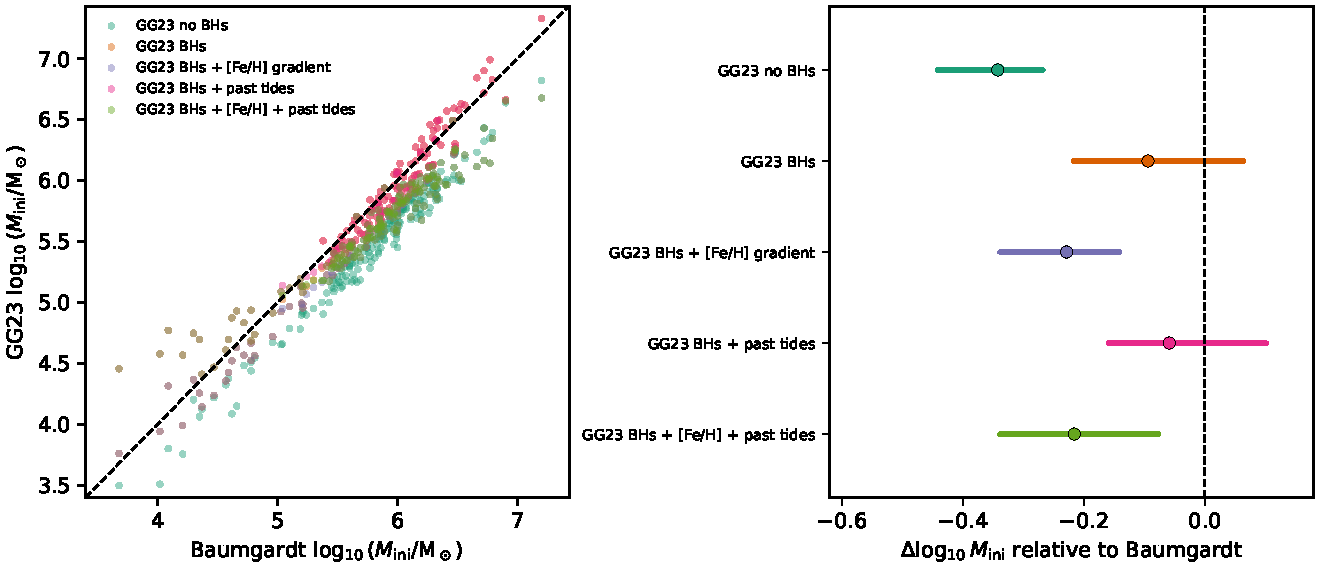
\includegraphics[width=\textwidth]{figures/gg23_initial_mass_model_comparison.pdf}
    \caption{Initial masses inferred by inverting the GG23 mass-loss law for the observed Milky Way GCs. Left: GG23-derived initial masses compared to the Baumgardt initial masses. The dashed line marks equality. Right: median and central 68 per cent range of $\Delta\log_{10}M_{\rm ini}=\log_{10}M_{\rm ini}^{\rm GG23}-\log_{10}M_{\rm ini}^{\rm Baumgardt}$ for each GG23 variant.}
    \label{fig:gg23_initial_mass_comparison}
\end{figure*}

We compute the corresponding GG23 survivability boundaries independently of the plotted points. For each cluster orbit we find the limiting mass $M_{\rm cut}$ satisfying
\begin{equation}
t_{\rm dis}(M_{\rm cut},R_{\rm eff},R)=12\,{\rm Gyr}.
\end{equation}
At each value of $\log a$ we then average the orbit-by-orbit survival indicators with a Gaussian kernel in $\log a$ of width $0.18$ dex:
\begin{equation}
S_{\rm raw}(m,a)
=
\left\langle
{\bf 1}\left[m\ge \log_{10}M_{\rm cut}\right]
\right\rangle_{\log a},
\qquad
m=\log_{10}M_{\rm ini}.
\end{equation}
Finally, we fit the same monotonic logistic-tail representation used for the Baumgardt survivability surface. The thick contours in Figure~\ref{fig:gg23_survivability_model_mini} are the fitted $S=0.5$ boundaries, while the thin contours show $S=0.1$ and $S=0.9$.

The important point is that Figure~\ref{fig:gg23_survivability_model_mini} changes only the dynamical mass-loss calibration. The background in each GG23 panel is the survivability implied by that GG23 law and the observed orbit distribution; the points in that panel are the same observed clusters, but plotted at the $M_{\rm ini}$ recovered from that same GG23 law. The surface is therefore not fitted to the plotted point cloud. It is the forward survival probability surface through which those transformed points would be observed.

\begin{figure*}
    \centering
    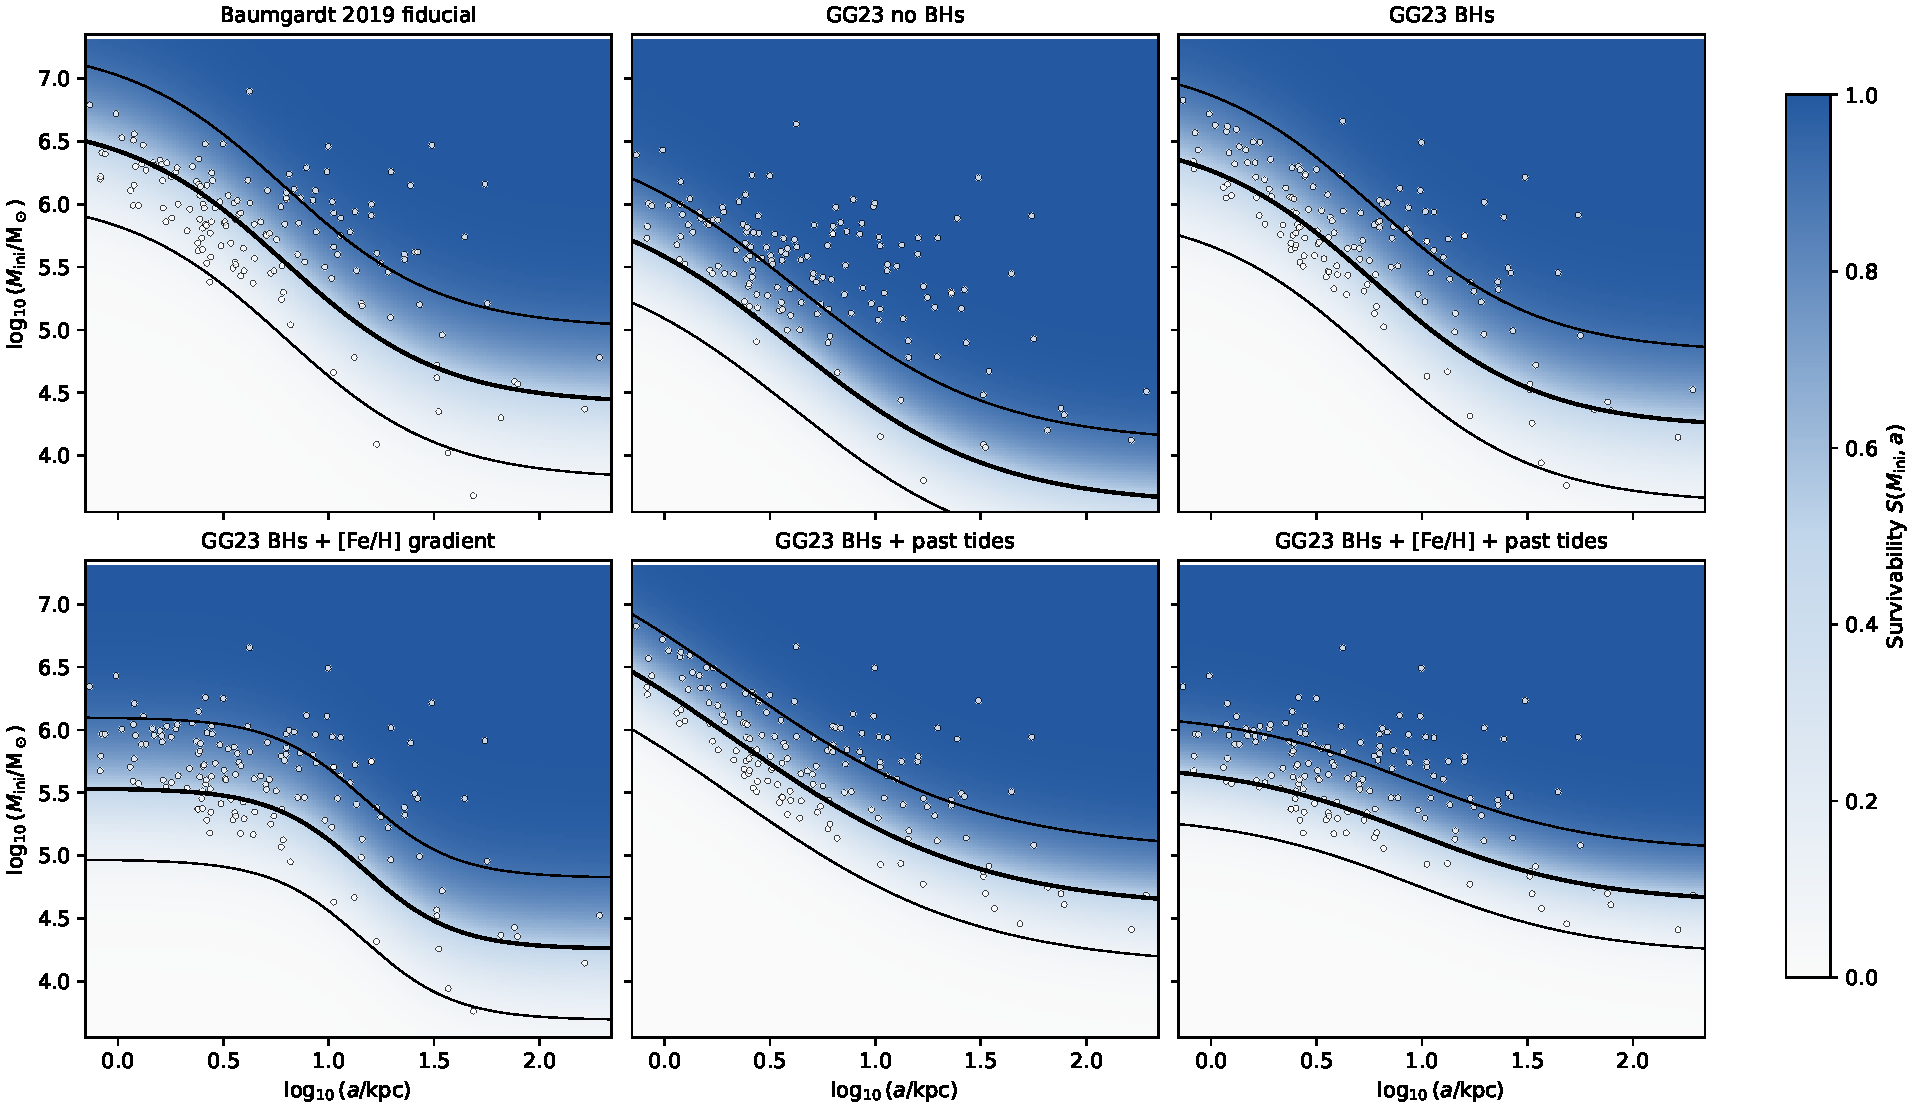
\includegraphics[width=\textwidth]{figures/gg23_survivability_maps_model_mini.pdf}
    \caption{Survivability surfaces under the Baumgardt and GG23 disruption calibrations. The Baumgardt panel uses the Baumgardt initial masses. Each GG23 panel uses initial masses obtained by inverting the corresponding GG23 mass-loss law for the observed present-day cluster mass and orbit. In all panels the background colour gives the fitted survivability surface $S(M_{\rm ini},a)$, the thick black curve marks $S=0.5$, and the thin curves mark $S=0.1$ and $S=0.9$.}
    \label{fig:gg23_survivability_model_mini}
\end{figure*}

We then repeat the exact single-component Schechter inference in each GG23 coordinate system, using the same $\texttt{logpoly3}$ radial family and the same iterative detectability correction. Figure~\ref{fig:gg23_imf_comparison} compares the resulting IMFs and posterior parameter distributions with the Baumgardt-based baseline, and Table~\ref{tab:gg23_imf_comparison} lists the corresponding inferred parameters. The alternative disruption laws change the preferred lower-bound population at the factor-of-two level, but they do not drive the fit to a qualitatively different IMF family. All six solutions remain Schechter-like over the constrained mass range. The largest shifts come from the metallicity-gradient and past-tidal-evolution variants, which change both the recovered initial masses of the observed clusters and the survivability correction applied below the present-day catalogue.

To compare the six disruption calibrations in a common observed space, we also compute a posterior predictive count likelihood for the binned present-day catalogue. The data vector contains counts in bins of $(\log M_{\rm now},\log a,D_\odot,|b|,|l|)$. For each posterior draw, we reconstruct the draw-specific survivability $S(M_{\rm ini},a)$ and intrinsic effective detectability $Q(M_{\rm ini},a)$, fix the Schechter IMF to the sampled $(\alpha,\log_{10}M_c)$ values, and reprofile the three nuisance coefficients of the $\texttt{logpoly3}$ radial law. We then predict the complete-survivor distribution in observable space, refit the logistic completeness law $C(\log M_{\rm now},D_\odot,|b|,|l|)$ for that draw, and evaluate the Poisson likelihood of the observed binned counts,
\begin{equation}
P_{\rm pred}
=
\left\langle
\prod_j
\frac{\mu_j(\theta)^{n_j}\exp[-\mu_j(\theta)]}{n_j!}
\right\rangle_{\theta},
\end{equation}
where $n_j$ is the observed count in bin $j$, $\mu_j(\theta)$ is the selected predicted count for posterior draw $\theta$, and the average is over posterior draws. The last column of Table~\ref{tab:gg23_imf_comparison} reports $\Delta\ln P_{\rm pred}$ relative to the best value among the six models. This is an observed-space posterior predictive diagnostic, not an independent held-out validation; it asks which fitted disruption calibration best reproduces the joint distribution of present-day mass, orbit size, sky position, and heliocentric distance after the same selection treatment is applied.

\begin{figure*}
    \centering
    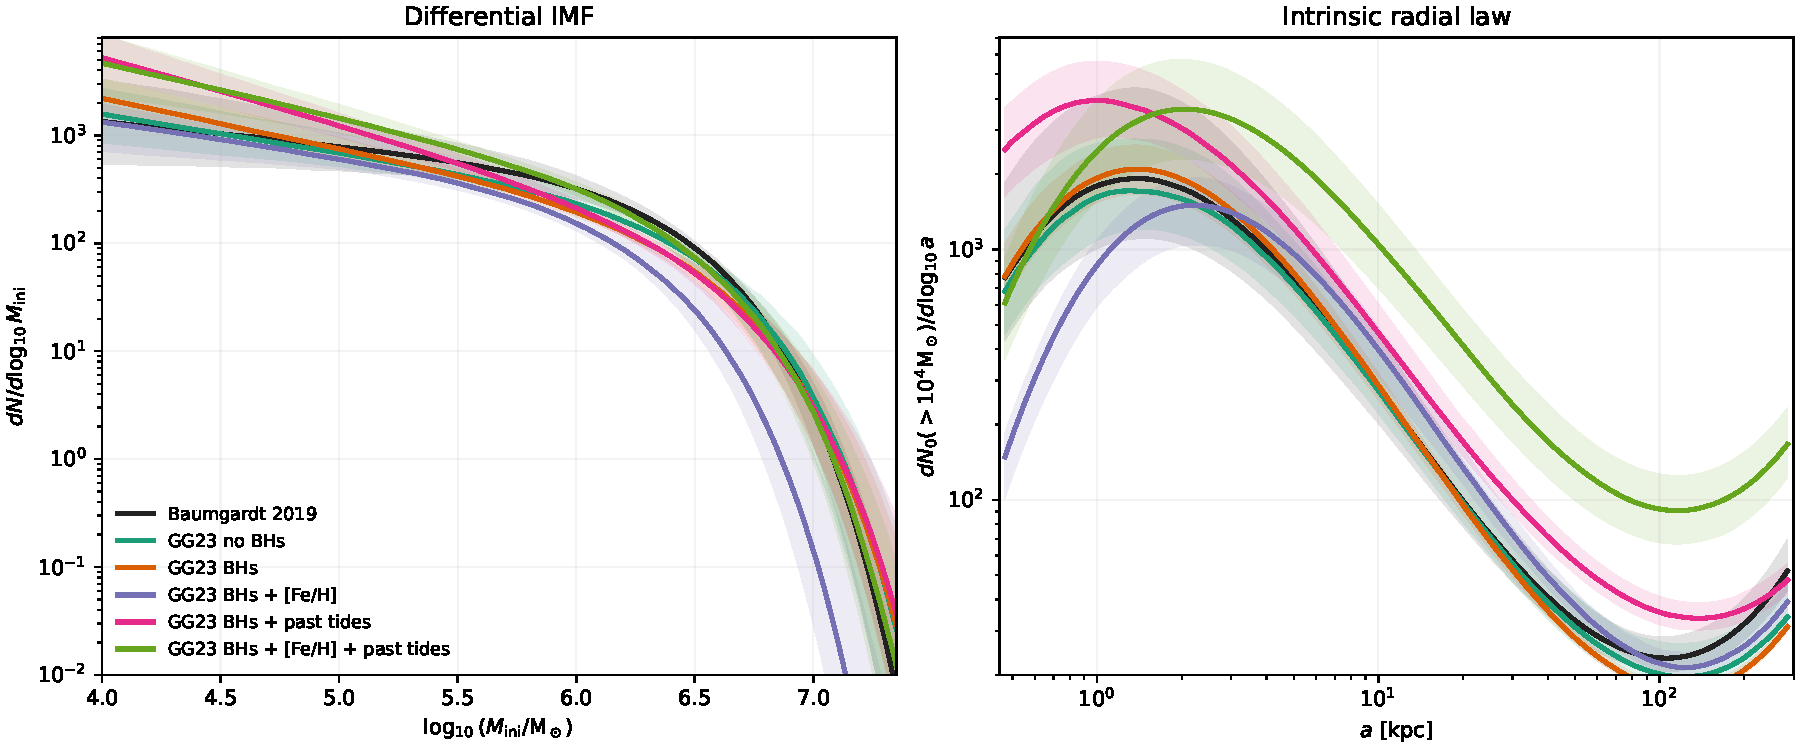
\includegraphics[width=\textwidth]{figures/gg23_imf_comparison.pdf}
    \caption{Inferred Schechter IMFs and posterior parameter distributions for the Baumgardt baseline and the five GG23 disruption calibrations. Left: differential IMF, $dN/d\log_{10}M_{\rm ini}$; solid curves show posterior medians and shaded bands show the central 68 per cent posterior ranges. Middle: posterior probability distributions in the Schechter-parameter plane $(\alpha,\log_{10}M_c)$. Right: posterior probability distributions in the birth-population plane $(N_0,M_{\star,0})$ for clusters born above $M_{\rm ini}=10^4\,{\rm M}_\odot$. Contours enclose 68 and 95 per cent of each posterior distribution, and points mark posterior medians. Each model uses the same $\texttt{logpoly3}$ radial family.}
    \label{fig:gg23_imf_comparison}
\end{figure*}

\begin{table*}
    \centering
    \caption{Inferred Schechter parameters for the Baumgardt baseline and the five GG23 disruption calibrations. Quoted values are posterior medians with central 68 per cent ranges. The $N_0$ and $M_{\star,0}$ columns give the inferred number and stellar mass of clusters born above $M_{\rm ini}=10^4\,{\rm M}_\odot$. The final column gives the posterior predictive log-likelihood difference in the binned observed space $(\log M_{\rm now},\log a,D_\odot,|b|,|l|)$, measured relative to the best of the six models. Rows are ordered by decreasing posterior predictive score.}
    \label{tab:gg23_imf_comparison}
    \begin{tabular}{lcccccc}
        \hline
        Model & $\eta_t$ & $\alpha$ & $\log_{10}(M_c/{\rm M}_\odot)$ & $N_0(>10^4)$ & $M_{\star,0}(>10^4)\,[10^8{\rm M}_\odot]$ & $\Delta\ln P_{\rm pred}$ \\
        \hline
                Baumgardt 2019 & 1.17$^{+0.32}_{-0.22}$ & -1.21$^{+0.16}_{-0.16}$ & 6.32$^{+0.09}_{-0.09}$ & 1722$^{+1479}_{-717}$ & 4.71$^{+1.52}_{-0.99}$ & -13.66 \\
        GG23 no BHs & 0.40$^{+0.10}_{-0.03}$ & -1.33$^{+0.14}_{-0.11}$ & 6.43$^{+0.15}_{-0.16}$ & 1576$^{+902}_{-450}$ & 3.73$^{+1.25}_{-0.41}$ & -9.96 \\
        GG23 BHs & 1.19$^{+0.10}_{-0.11}$ & -1.45$^{+0.08}_{-0.09}$ & 6.46$^{+0.14}_{-0.10}$ & 1823$^{+681}_{-330}$ & 3.32$^{+0.46}_{-0.42}$ & -8.09 \\
        GG23 BHs + [Fe/H] & 0.77$^{+0.11}_{-0.15}$ & -1.30$^{+0.18}_{-0.13}$ & 6.16$^{+0.15}_{-0.10}$ & 1346$^{+395}_{-355}$ & 2.24$^{+0.67}_{-0.38}$ & -4.20 \\
        GG23 BHs + past tides & 1.19$^{+0.13}_{-0.07}$ & -1.63$^{+0.09}_{-0.09}$ & 6.50$^{+0.17}_{-0.13}$ & 3467$^{+1499}_{-935}$ & 4.13$^{+0.79}_{-0.72}$ & -8.87 \\
        GG23 BHs + [Fe/H] + past tides & 0.48$^{+0.06}_{-0.06}$ & -1.49$^{+0.17}_{-0.16}$ & 6.39$^{+0.15}_{-0.13}$ & 3674$^{+1815}_{-1278}$ & 5.40$^{+1.24}_{-0.95}$ & 0.00 \\

    \end{tabular}
\end{table*}

\clearpage

\section{Discussion}\label{sec:discussion}

\subsection{Comparison with previous constraints on the initial GC mass function}\label{sec:discussion_literature}
The result of Section~\ref{sec:single_component_results} places the Milky Way in the family of Schechter-like GCIMF models, but with an important qualification: the inferred cutoff is the cutoff required after applying the adopted survivability and detectability filters. It should therefore not be read as a direct measurement of the maximum cluster mass at birth. In this sense our result sits between the two limiting pictures discussed in the Introduction. It does not require the present-day GCMF turnover to have been fully primordial, as in lognormal or gas-expulsion models, but neither does it infer the GCIMF from the present-day mass function alone. The fitted normalization and $M_{\rm c}$ are conditional on the orbit-dependent survival boundary in the $(M_{\rm ini},a)$ plane.

\subsection{A lower bound on the initial GC population}\label{sec:lower_bound}
The present analysis constrains the progenitors of the \emph{surviving} Milky Way GC family. It does not constrain a completely destroyed population that leaves no surviving counterpart in the current catalogue. In that sense the fitted normalization is intentionally conservative: it is the number of progenitors required to explain the observed survivors once survivability and detectability are treated self-consistently, not the total number of clusters that may once have formed in the proto-Milky Way.

This limitation is clearest in the inner Galaxy. The fitted survivability surface still rises steeply toward small semimajor axis, and the present data provide little direct leverage on clusters that were destroyed before the present epoch. The reported normalization should therefore be interpreted as a lower bound tied to the surviving Milky Way GC family above $M_{\rm ini}=10^4\,{\rm M}_\odot$.

\section{Conclusions}\label{sec:conclusion}
The main results of this draft are as follows.
\begin{enumerate}
    \item The Milky Way GC catalogue can be modelled directly as a Poisson point process in the $(\log M_{\rm ini},\log a)$ plane, with an intrinsic Schechter IMF and a radial birth profile filtered by survivability and detectability.
    \item The adopted survivability surface is a smooth logistic-tail transition in $\log M_{\rm ini}$ at fixed semimajor axis, calibrated to the orbit-based dissolution-time model through the $S=0.1$, $0.5$, and $0.9$ contours.
    \item In the adopted exact single-component model, the best-fit outer parameters are $\eta_t=\ExactBestEta$, $\alpha=\ExactBestAlpha$, and $\log_{10}(M_c/{\rm M}_\odot)=\ExactBestMc$, with posterior medians $\eta_t=\PosteriorEtaMed_{-\PosteriorEtaMinus}^{+\PosteriorEtaPlus}$, $\alpha=\PosteriorAlphaMed_{-\PosteriorAlphaMinus}^{+\PosteriorAlphaPlus}$, and $\log_{10}(M_c/{\rm M}_\odot)=\PosteriorMcMed_{-\PosteriorMcMinus}^{+\PosteriorMcPlus}$.
    \item Above $M_{\rm ini}=10^4\,{\rm M}_\odot$, the inferred initial GC population is $N_0=\PosteriorNzeroMed_{-\PosteriorNzeroMinus}^{+\PosteriorNzeroPlus}$, corresponding to $M_{\star,0}=\PosteriorMassZeroEightMed_{-\PosteriorMassZeroEightMinus}^{+\PosteriorMassZeroEightPlus}\times10^8\,{\rm M}_\odot$.
    \item The detectability correction is moderate: at fixed Schechter parameters it raises the baseline normalization by a factor of \ExactCountRatio.
    \item Among the tested radial families, the smooth $\texttt{logpoly3}$ model is preferred over the five-bin step model, a single power law in $a$, and a cored power law in $a$, even after the information-criterion penalty for additional flexibility is included.
    \item All quoted normalizations remain lower bounds. The present analysis cannot constrain a completely destroyed GC population in the inner Galaxy, and the reported totals refer only to the progenitors of the surviving GC family anchored by the observed catalogue.
\end{enumerate}

\section*{Data availability}
All figures, tables, and scripts used in this draft are stored locally in the project directory. The Baumgardt source tables are saved under \texttt{data/raw/}, the processed catalogues are under \texttt{data/processed/}, and the paper-ready single-component figures and summary tables are regenerated by \path{scripts/build_paper_assets_exact_single_component.py}.

\bibliographystyle{mnras}
\bibliography{references}

\bsp
\label{lastpage}
\end{document}
